% ===========================================================================
% BRCA Multi-Omics Data Mining — Academic Paper
% Version: 0518-1153  (captions verified against actual plotting code)
% ===========================================================================
\documentclass[12pt,a4paper]{ctexart}

\usepackage[top=2.5cm, bottom=2.5cm, left=3cm, right=2.5cm]{geometry}
\usepackage{graphicx}
\usepackage{booktabs}
\usepackage[labelfont=bf,font=small]{caption}
\usepackage[hidelinks]{hyperref}
\usepackage{amsmath}
\usepackage{float}
\usepackage{array}
\usepackage{multirow}
\usepackage{listings}
\usepackage{xcolor}

\lstset{basicstyle=\ttfamily\footnotesize,breaklines=true,frame=single,numbers=left,numberstyle=\tiny,backgroundcolor=\color{gray!5}}

\usepackage[backend=biber,style=gb7714-2015]{biblatex}
\addbibresource{references.bib}
\graphicspath{{../../results/figures_pub/}}

\title{\heiti\zihao{3} 基于多组学数据挖掘的乳腺癌分子特征分析}
\author{}
\date{}

\begin{document}

\maketitle

% ==================== 摘要 ====================
\begin{abstract}
\noindent
乳腺癌是全球发病率最高的恶性肿瘤，其分子异质性是精准诊疗面临的核心挑战。本研究基于TCGA-BRCA多组学数据（mRNA转录组25,981个基因、miRNA表达谱1,881个、体细胞突变15,413个基因及临床注释94项），对1,076例多组学共同患者进行了系统性的数据挖掘分析。研究综合运用DESeq2差异表达分析、LASSO和随机森林分类、PCA/t-SNE聚类、WGCNA共表达网络、Cox比例风险回归、maftools突变景观分析、g:Profiler功能富集分析、arules关联规则挖掘及ConsensusClusterPlus共识聚类等算法。主要结果包括：鉴定6,768个显著差异表达基因（$|\log_2\text{FC}|>1$, FDR$<0.05$），其中上调4,334个、下调2,434个；LASSO分类器以89.4\%准确率实现三分类分子亚型预测，仅使用35个基因；WGCNA识别9个共表达模块，blue模块枢纽基因模块隶属度达0.959；Cox模型C-index为0.771，Stage IV风险比达8.74；PIK3CA（37.3\%）和TP53（35.2\%）为最高频突变基因；功能富集揭示上调基因显著富集于细胞周期通路（Reactome Cell Cycle, 187个基因, $p=1.5\times10^{-21}$）。本研究为乳腺癌多组学数据挖掘提供了完整分析框架。

\vspace{1em}
\noindent\textbf{关键词}：乳腺癌；TCGA；多组学数据挖掘；差异表达分析；WGCNA；预后模型
\end{abstract}

\newpage

% ==================== 1 引言 ====================
\section{引言}

\subsection{研究背景}

据国际癌症研究机构（IARC）GLOBOCAN 2022统计，全球每年新发癌症约2,000万例，死亡约970万例\cite{sung2024global}。其中女性乳腺癌以约230万例新发病例居全球恶性肿瘤发病率首位，同年导致约67万例死亡。在中国，乳腺癌的发病率和死亡率持续上升，且发病年龄显著早于欧美国家。

乳腺癌的发生发展涉及多基因突变累积、表观遗传重塑及信号通路交互失调等复杂的分子过程\cite{hanahan2011hallmarks}。传统单一维度研究方法难以全面揭示乳腺癌的系统性分子特征。以癌症基因组图谱（The Cancer Genome Atlas, TCGA）\cite{tcga2012comprehensive}为代表的国际大型合作项目提供了涵盖多组学的海量公开数据。在此背景下，数据挖掘技术为从高维度组学数据中提取具有生物学和临床价值的信息提供了方法论支撑。

\subsection{乳腺癌分子分型}

乳腺癌是由多种分子特征各异的亚型构成的异质性疾病集合。Perou等\cite{perou2000molecular}于2000年首次提出乳腺癌分子分型体系，目前广泛认可的固有分子亚型包括四类：Luminal A型（50\%--60\%，ER+/PR+/HER2-/Ki-67低表达），Luminal B型（15\%--20\%），HER2过表达型（10\%--15\%），三阴性型（15\%--20\%）。尽管该体系已广泛用于临床，同一亚型内部的生物学异质性仍然显著，整合多组学数据进一步挖掘分子分型的内在结构具有重要的研究价值。

\subsection{数据挖掘在癌症研究中的应用}

在差异表达分析方面，DESeq2\cite{love2014moderated}基于负二项分布对RNA-seq计数数据建模。WGCNA\cite{langfelder2008wgcna}通过构建无标度拓扑网络将基因聚类为共表达模块。LASSO-Cox\cite{simon2011regularization}能有效应对高维数据中的维数灾难。g:Profiler\cite{kolberg2023gprofiler}提供一站式多数据库功能富集。Apriori算法\cite{agrawal1994fast}可从离散化数据中挖掘关联规则。共识聚类\cite{wilkerson2010consensus}通过重采样评估聚类稳定性。

\subsection{研究目的与论文结构}

本研究以TCGA-BRCA多组学数据为对象，综合运用多种数据挖掘方法，系统分析乳腺癌的分子特征。论文结构如下：第2章介绍材料与方法；第3章呈现分析结果；第4章为讨论；第5章给出结论；附录提供核心R代码。

% ==================== 2 材料与方法 ====================
\section{材料与方法}

\subsection{数据来源}

本研究数据来源于TCGA-BRCA队列。所有数据通过TCGAbiolinks R包\cite{colaprico2016tcgabiolinks}从GDC API获取（GDC Data Release 42.0），涵盖四个数据层：
（1）mRNA转录组（HiSeq RNA-seq, STAR-Counts流程）：原始计数矩阵包含60,660个基因；
（2）miRNA转录组（HiSeq miRNA-seq, BCGSC miRNA Profiling）：1,881个miRNA；
（3）体细胞突变（WES, MuTect2流程）：MAF格式突变注释文件；
（4）临床信息：94个原始变量。

\subsection{数据预处理}

\textbf{mRNA数据预处理}：低表达过滤标准为至少在10\%样本中counts $\geq$ 10，保留25,981个基因（42.8\%）。采用TPM归一化，基因标识符通过org.Hs.eg.db建立Ensembl ID到Gene Symbol的映射。临床数据提取25个核心变量，分子亚型根据ER/PR/HER2免疫组化状态分类。缺失值：数值型采用中位数填补，分类型采用众数填补。miRNA数据全部保留，突变数据经maftools\cite{mayakonda2018maftools}加载和质控。

\textbf{多组学整合}：提取各数据层样本条形码前12个字符作为患者ID，取交集确定1,076例核心患者队列。

\subsection{分析方法}

\textbf{差异表达分析}：采用DESeq2\cite{love2014moderated}进行肿瘤vs正常（$n=1,105$, $n=113$）和TN vs Luminal A（$n=115$, $n=950$）的差异表达分析，阈值FDR $<0.05$且$|\log_2\text{FC}|>1$。

\textbf{功能富集分析}：采用g:Profiler（gprofiler2 R包）\cite{kolberg2023gprofiler}，覆盖GO:BP、GO:MF、GO:CC、KEGG、Reactome和WikiPathway（FDR $<0.05$，排除IEA）。

\textbf{分类}：LASSO（5折交叉验证，$\alpha=1$）、随机森林（ntree=500）、XGBoost（nrounds=100）。输入为Top 500可变基因$\log_2(\text{TPM}+1)$，7:3分层划分。

\textbf{聚类}：PCA（Top 2,000基因中心化标准化）、t-SNE（perplexity=30）、K-means（$K=2$--10，轮廓系数）、共识聚类（80\%重采样，1,000次迭代）\cite{wilkerson2010consensus}。

\textbf{WGCNA}\cite{langfelder2008wgcna}：Top 5,000可变基因，signed网络，minModuleSize=30，mergeCutHeight=0.25。

\textbf{生存分析}：Kaplan-Meier（log-rank）、多变量Cox（C-index、似然比检验）、3年生存列线图（rms包）。

\textbf{突变分析}：maftools\cite{mayakonda2018maftools}，TMB按每兆碱基计算（WES $\approx$38 Mb）。

\textbf{关联规则}：Apriori（支持度0.3，置信度0.7）。miRNA-mRNA网络：Pearson相关（$|r|>0.4$）。

\subsection{分析环境}

R 4.6.0 + Bioconductor 3.23，Windows 11。主要R包：DESeq2、gprofiler2、caret、randomForest、glmnet、WGCNA、survival、survminer、rms、maftools、arules、ConsensusClusterPlus、ggplot2、ggsci、pheatmap。论文编译：MiKTeX 25.12 + XeLaTeX。

% ==================== 3 结果 ====================
\section{结果}

\subsection{数据概览}

经预处理和跨组学整合，最终分析数据集概况见表\ref{tab:data}。mRNA覆盖1,094例肿瘤（另113例正常），miRNA覆盖1,079例。多组学对齐后获得1,076例共同患者（重叠率98.4\%），突变数据覆盖990例（983例患者）。临床特征中Luminal A占绝对优势（950例，86.3\%），HER2-enriched仅37例（3.4\%），Triple Negative 115例（10.4\%）；Stage II占比最高（58.9\%），Stage IV仅20例（1.8\%）。中位OS随访约2.7年，死亡事件87例（7.9\%），事件率偏低是后续预后模型构建面临的核心约束。

\begin{table}[H]
\centering
\caption{多组学数据集总览}
\label{tab:data}
\begin{tabular}{llll}
\toprule
数据层 & 平台 & 特征数 & 样本量 \\
\midrule
mRNA表达 & HiSeq RNA-seq & 25,981 genes & 1,094 + 113 normal \\
miRNA表达 & HiSeq miRNA-seq & 1,881 miRNAs & 1,079 \\
体细胞突变 & WES (MuTect2) & 15,413 genes & 990 \\
临床数据 & TCGA Clinical & 25 variables & 1,174 \\
\bottomrule
\end{tabular}
\end{table}

\subsection{差异表达与功能富集}

\subsubsection{Tumor vs Normal 差异表达}

DESeq2在肿瘤（$n=1,105$）与正常（$n=113$）组织间共鉴定6,768个显著差异表达基因（$|\log_2\text{FC}|>1$, FDR$<0.05$），其中肿瘤相对正常上调4,334个、下调2,434个（表\ref{tab:deg}）。上调基因数量为下调的1.78倍，提示肿瘤细胞中转录激活事件的广泛性——已知癌症转录组以代谢重编程、细胞周期激活和增殖信号增强为特征，上调偏倚与这些过程的全局性激活一致。

图\ref{fig:volcano}以火山图展示了全部25,981个基因的分布格局。横轴为$\log_2$ Fold Change（截断$\pm6$），纵轴为$-\log_{10}(p)$（截断50）。两条虚线分别标记$|\log_2\text{FC}|=1$和$p=0.05$的显著性阈值。上调侧横坐标在2--5范围内的散点密度远高于下调侧对称位置。分布在图的远右侧（$\log_2\text{FC}>4$）且$-\log_{10}(p)>20$的区域代表在肿瘤中高度过表达且统计学证据极强的候选生物标志物。图中标注了差异最显著的若干基因的Gene Symbol以辅助识别。

\begin{figure}[H]
\centering
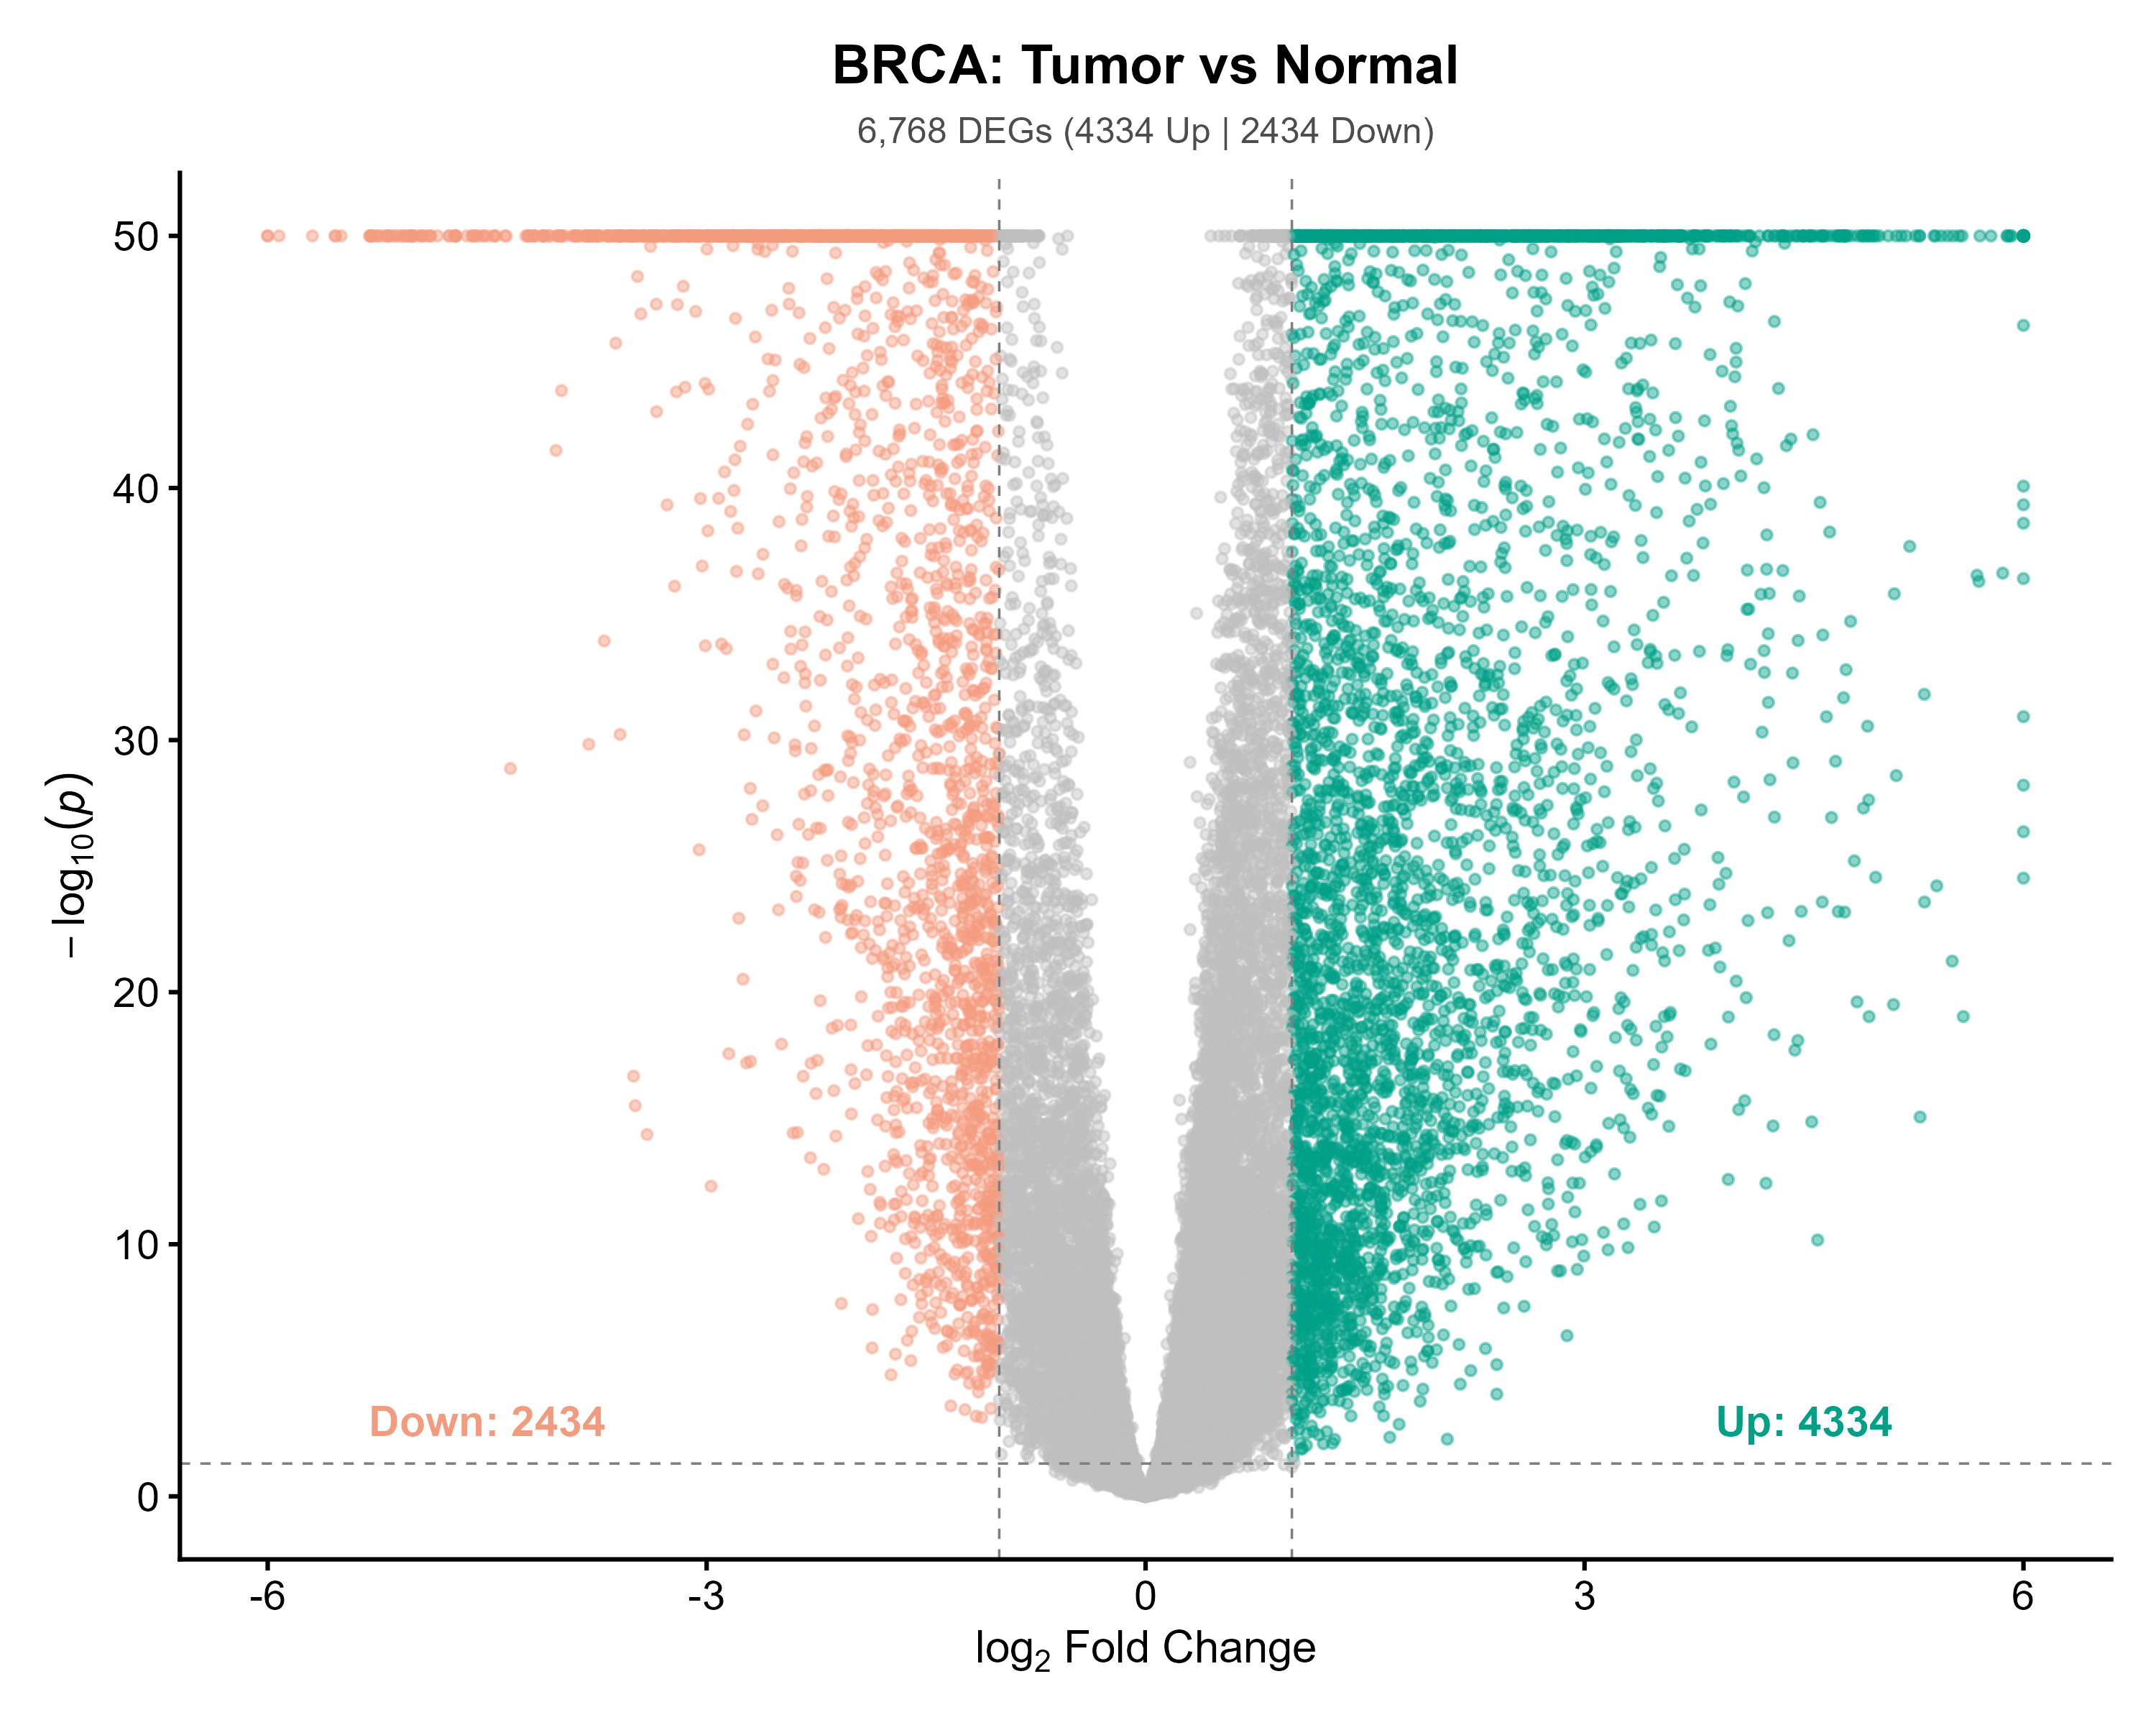
\includegraphics[width=0.85\textwidth]{fig1_volcano.png}
\caption{差异表达火山图（Tumor vs Normal）。横轴$\log_2$FC（$\pm6$），纵轴$-\log_{10}(p)$（50）。虚线上方且虚线外侧的点为满足$|\log_2\text{FC}|>1$且FDR$<0.05$的显著差异表达基因。NPG色板标注上调与下调方向。绘图参数：上调npg10[3]，下调npg10[5]，非显著grey75。}
\label{fig:volcano}
\end{figure}

\begin{table}[H]
\centering
\caption{差异表达分析结果}
\label{tab:deg}
\begin{tabular}{ll}
\toprule
指标 & 数值 \\
\midrule
总DEGs（$|\log_2\text{FC}|>1$, FDR$<0.05$） & 6,768 \\
上调基因数 & 4,334 \\
下调基因数 & 2,434 \\
分析方法 & DESeq2 (Wald test, BH correction) \\
\bottomrule
\end{tabular}
\end{table}

\subsubsection{亚型间差异表达}

Triple Negative（$n=115$）与Luminal A（$n=950$）之间的差异表达分析鉴定出4,888个显著基因（$|\log_2\text{FC}|>1$, FDR$<0.05$），其中TN上调2,270个，Luminal A上调2,618个（图\ref{fig:tnla}）。这一数字与Tumor vs Normal差异基因总数（6,768）处于同一数量级，说明两种极端分子亚型之间的转录组差异幅度不亚于肿瘤与正常组织的差异——这表明在乳腺癌内部，不同亚型代表了本质上不同的转录组状态，而非同一状态的细微调变。在TN中高表达的基因可优先作为TNBC潜在治疗靶点的候选来源。

\begin{figure}[H]
\centering
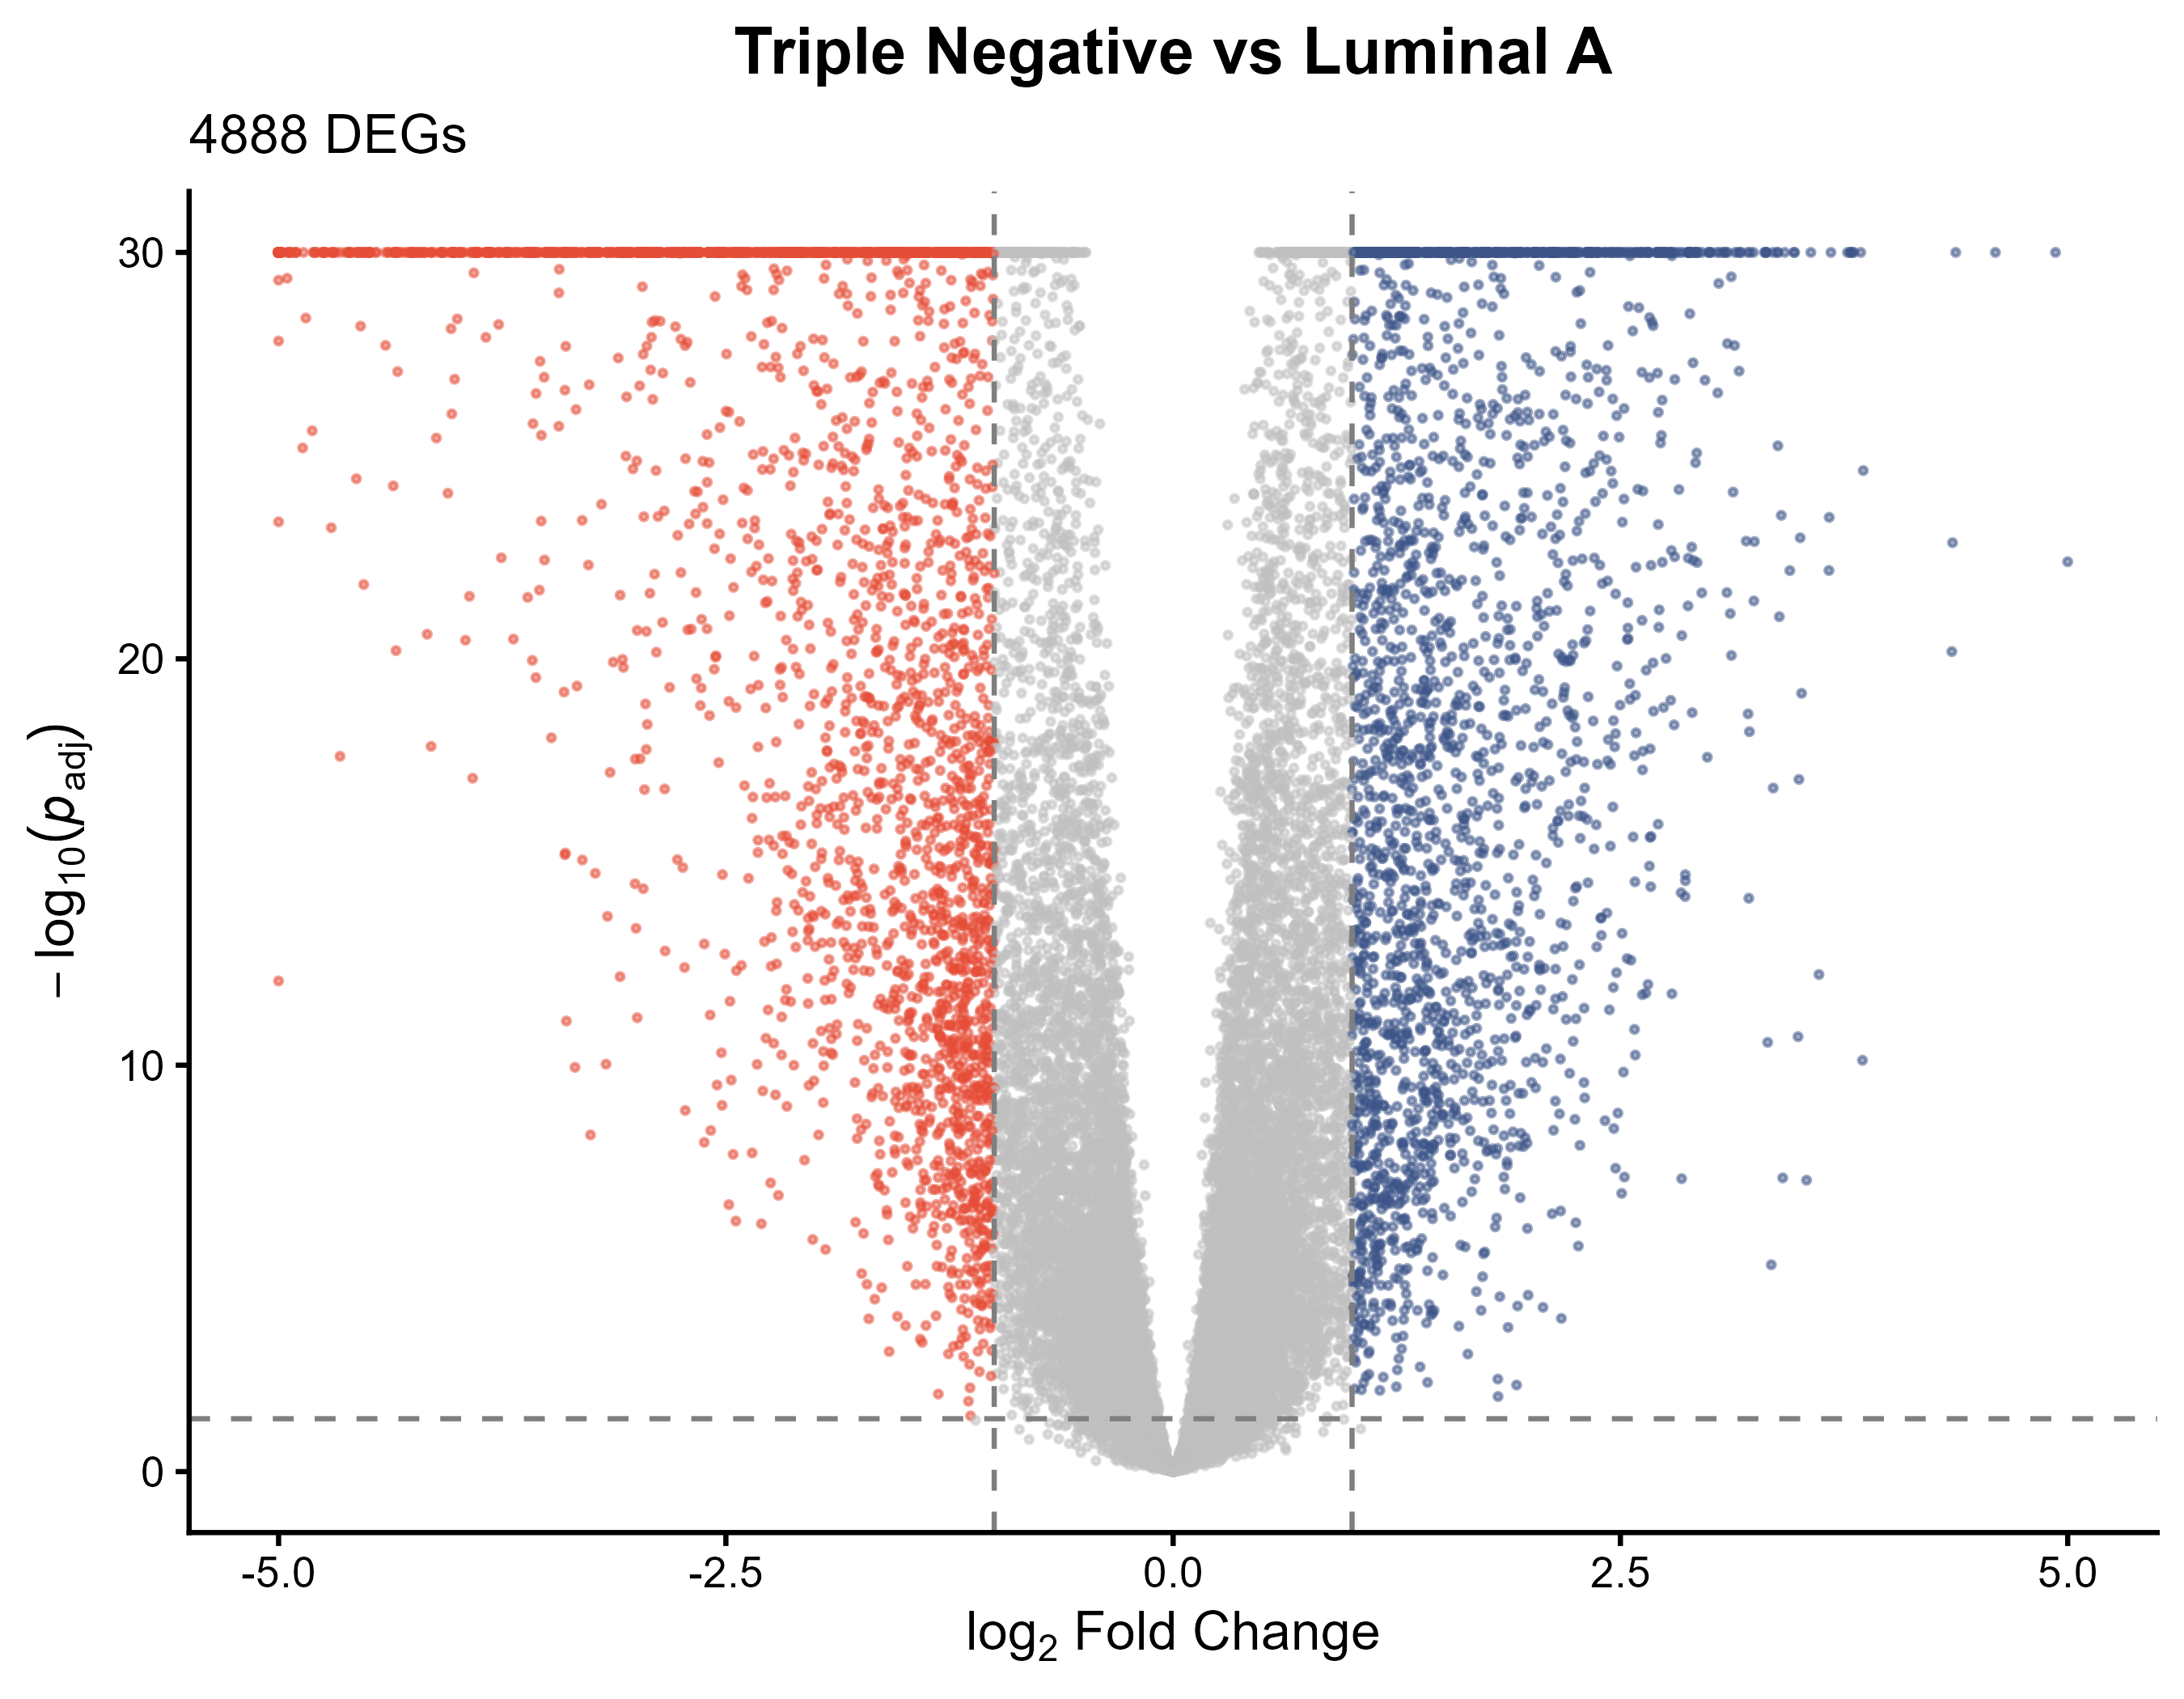
\includegraphics[width=0.85\textwidth]{fig17_tn_vs_la_volcano.png}
\caption{TN vs Luminal A差异表达火山图。横轴$\log_2$FC（$\pm5$），纵轴$-\log_{10}(p_{\text{adj}})$（30）。绘图参数：TN中上调npg10[4]，Luminal A中上调npg10[1]，非显著grey75。}
\label{fig:tnla}
\end{figure}

\subsubsection{功能富集分析}

上调基因的富集信号呈现高度集中的特征（图\ref{fig:enrich_up}）。在643条显著条目（FDR$<0.05$）中，前五位全部来自Reactome数据库，且功能主题高度一致：Cell Cycle（187个基因，$p=1.5\times10^{-21}$）以压倒性的显著性居首，其后依次为Cell Cycle Mitotic（160个基因）、Nucleosome Assembly、DNA Replication和Mitotic Chromosome Condensation。这五个通路共同指向BRCA肿瘤中转录激活最剧烈的事件是DNA复制和染色体分离机器。富集分析覆盖六个来源数据库：GO:BP（303条）、Reactome（191条）、GO:CC（75条）、GO:MF（37条）、WikiPathway（21条）和KEGG（16条），GO:BP条目数量最多但Reactome前五位通路显著性最强。

下调基因的富集方向截然不同（图\ref{fig:enrich_down}）。1,414条显著条目（数量为上调的两倍以上）分布更为广泛，主要集中于ECM organization、Cell adhesion、脂质代谢及PI3K-Akt信号通路。下调条目总数远超上调（1,414 vs 643），暗示被抑制的生物学功能类别比被激活的更为分散——这可能反映了肿瘤为存活需要在多种正常功能上妥协的生物学现实。表\ref{tab:enrich}汇总了三组基因集的富集统计。

\begin{figure}[H]
\centering
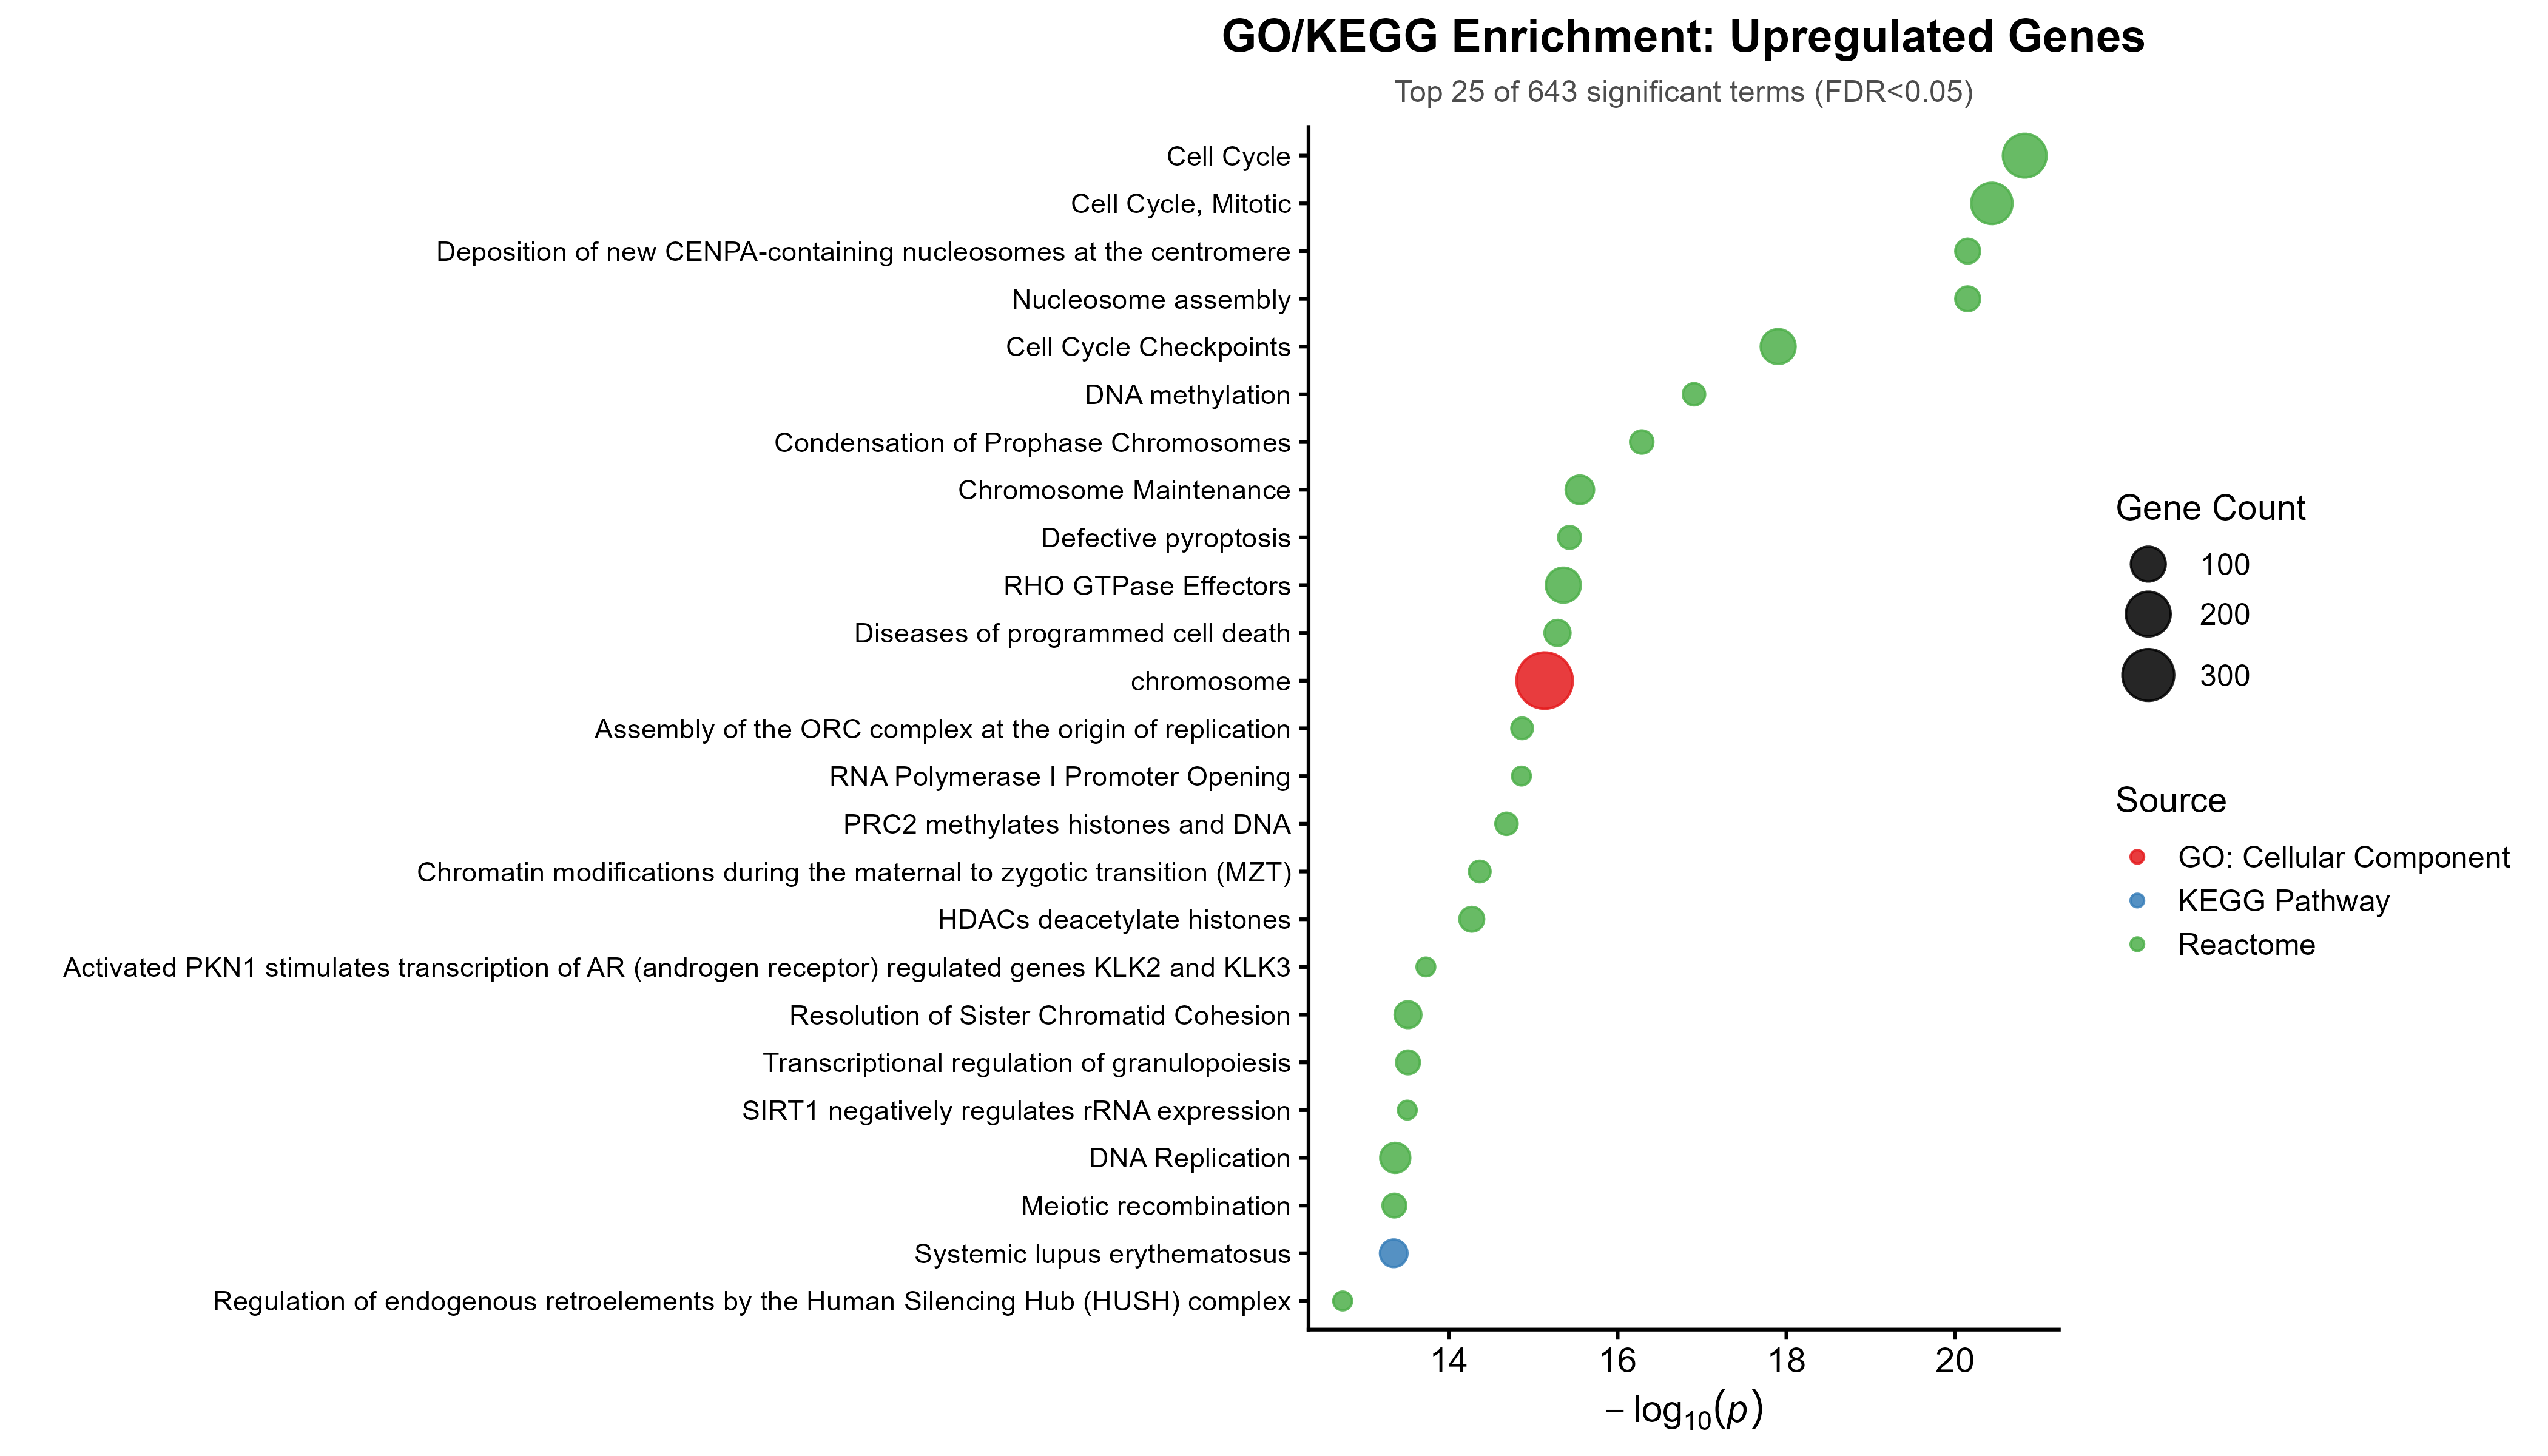
\includegraphics[width=0.85\textwidth]{fig12_enrichment_up.png}
\caption{上调基因富集气泡图（Top 25, FDR$<0.05$）。横轴$-\log_{10}(p)$，纵轴通路名称（按显著性降序）。气泡大小=交叠基因数量，颜色区分来源数据库（scale\_color\_brewer(palette="Set1")，覆盖GO:BP/MF/CC、KEGG、Reactome、WikiPathway六类）。前五位全部为Reactome条目。}
\label{fig:enrich_up}
\end{figure}

\begin{figure}[H]
\centering
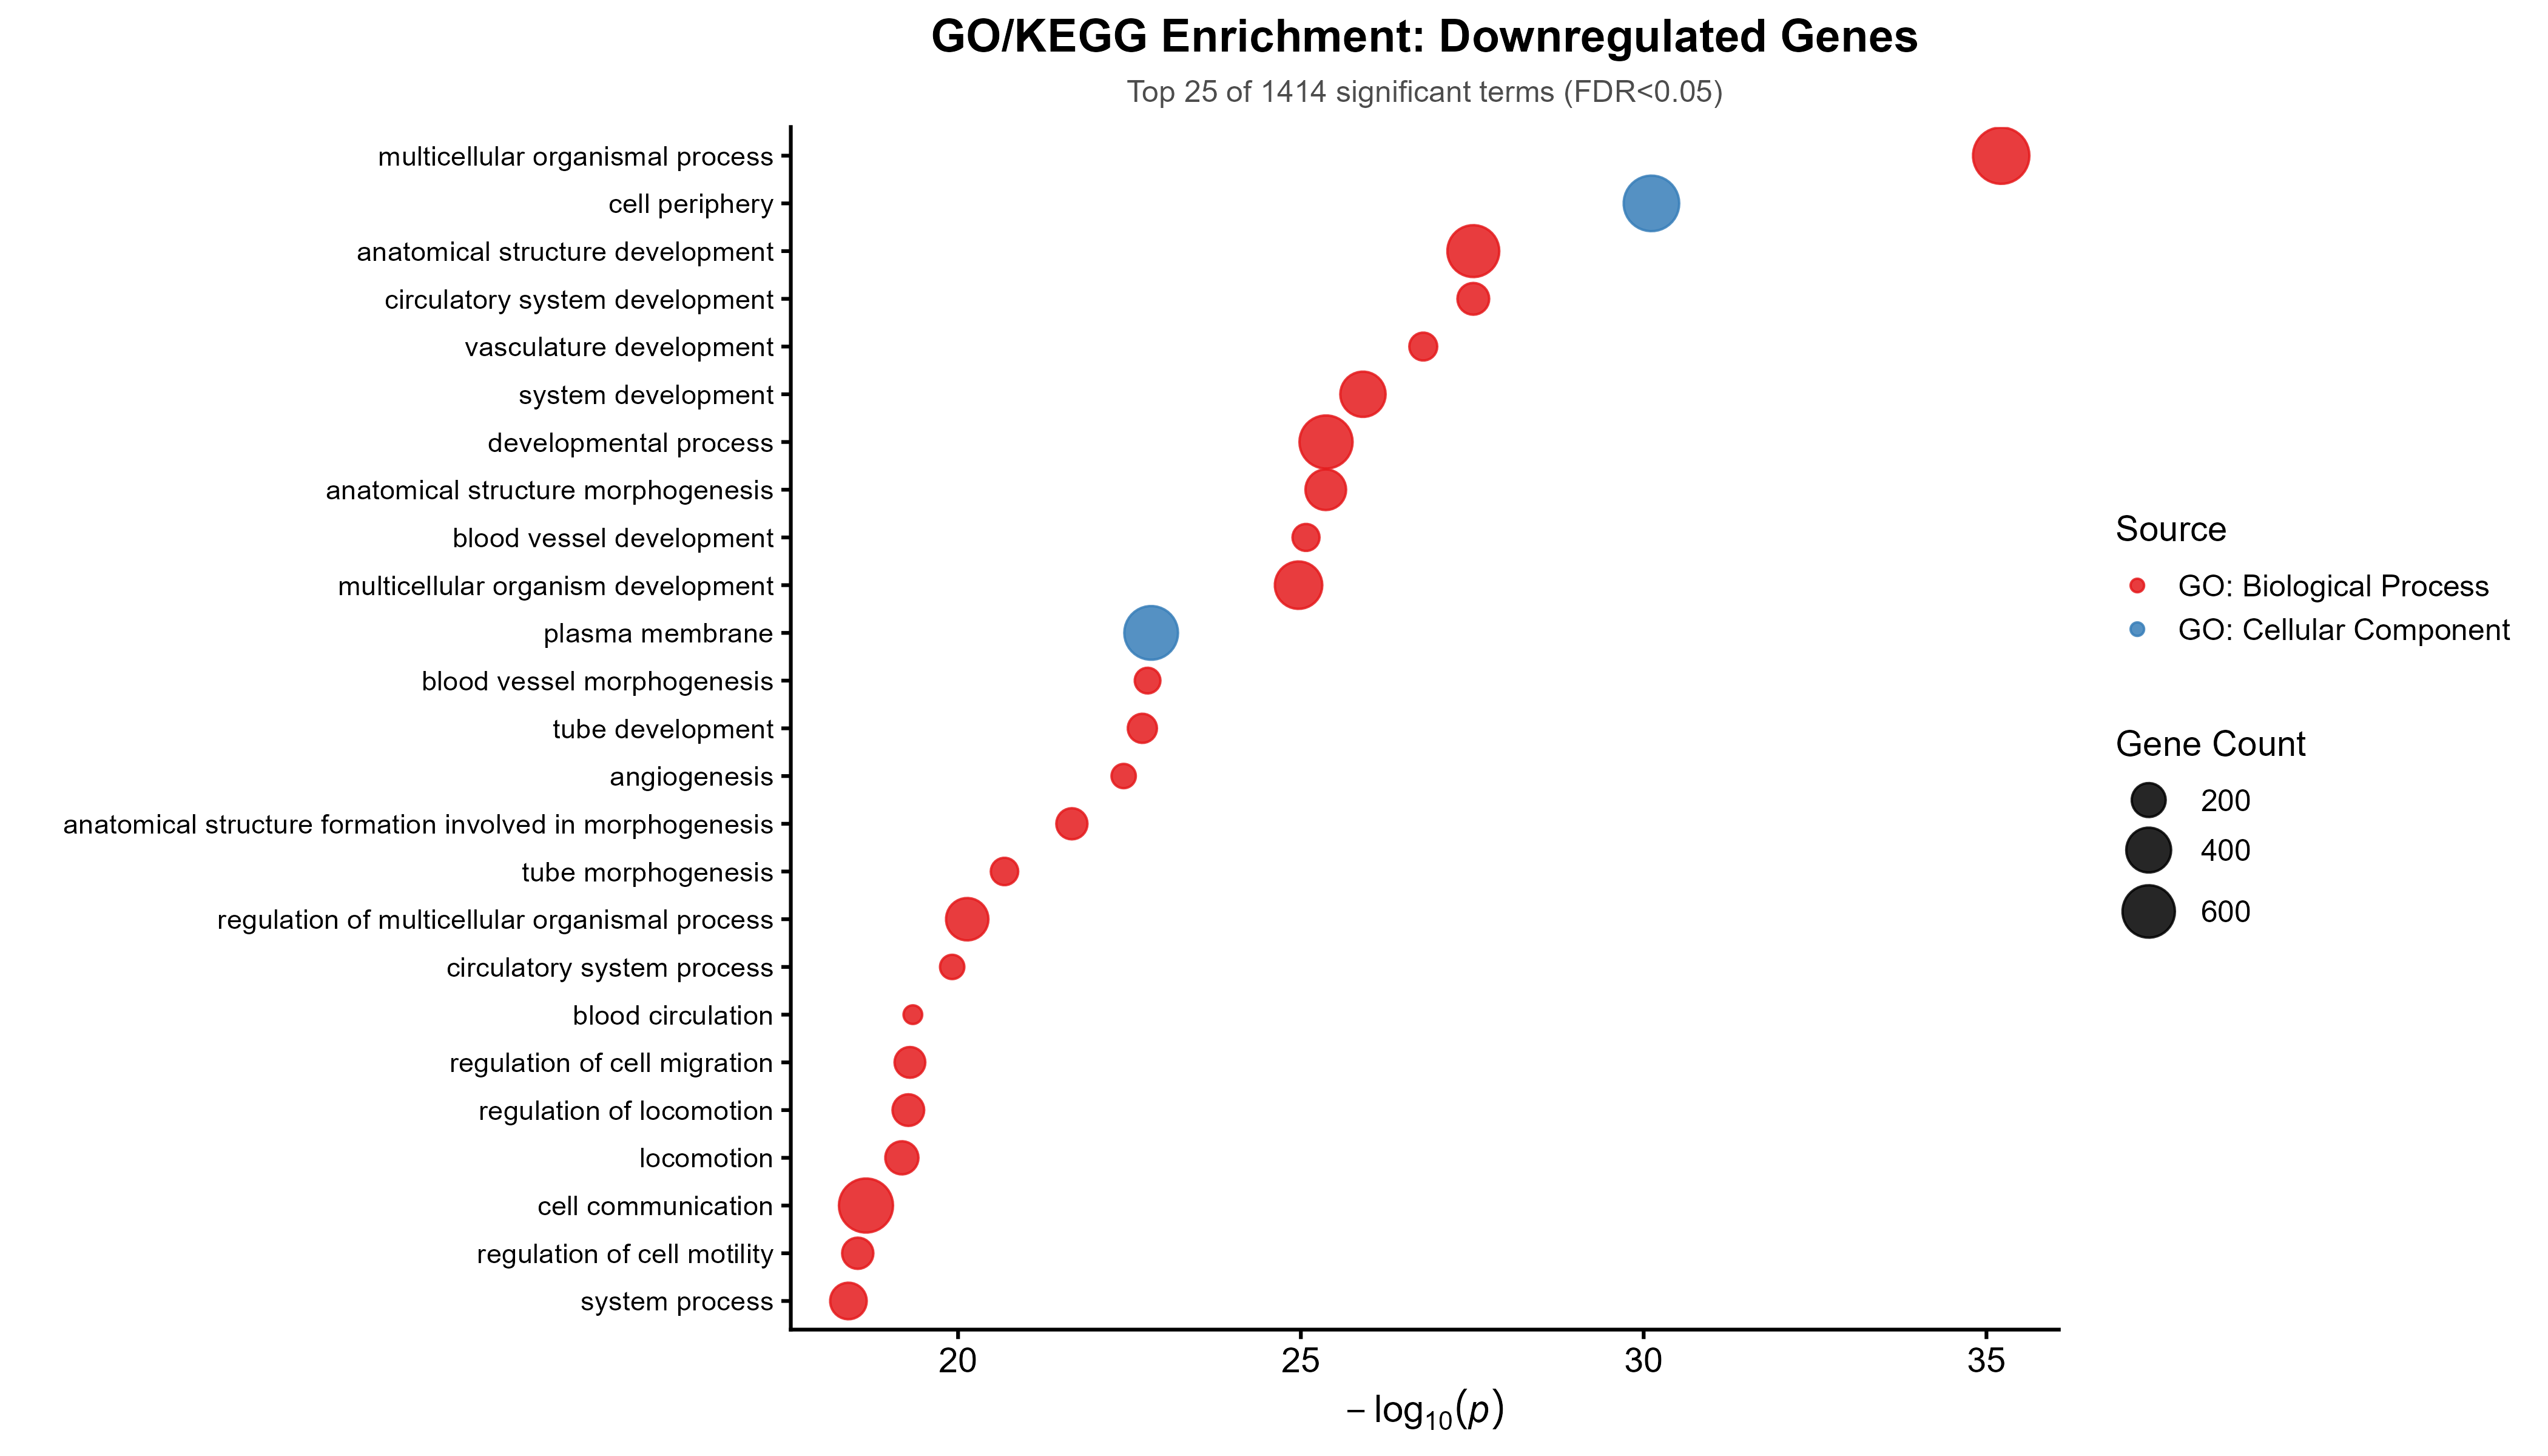
\includegraphics[width=0.85\textwidth]{fig13_enrichment_down.png}
\caption{下调基因富集气泡图（Top 25, FDR$<0.05$）。参数同上调图。分布较上调基因广泛，ECM organization和Cell adhesion占据显著位置。下调条目总数（1,414）超过上调（643）的两倍。}
\label{fig:enrich_down}
\end{figure}

\begin{table}[H]
\centering
\caption{功能富集分析结果汇总}
\label{tab:enrich}
\begin{tabular}{lllll}
\toprule
基因集 & 基因数 & 显著条目 & Top通路 & $p$值 \\
\midrule
上调 & 4,334 & 643 & Cell Cycle (Reactome) & $1.5\times10^{-21}$ \\
下调 & 2,434 & 1,414 & ECM Organization (Reactome) & $\sim10^{-15}$ \\
全部DEGs & 6,768 & 1,280 & Cell Cycle (Reactome) & $\sim10^{-18}$ \\
\bottomrule
\end{tabular}
\end{table}

\subsection{分子亚型分类}

三种分类器在独立测试集上的性能差异显著（图\ref{fig:model}，表\ref{tab:class}）。LASSO以89.4\%准确率排序第一（Kappa=0.528），且仅使用了从500个候选基因中筛选出的35个区分性基因——压缩比约为14:1。这一高压缩比说明决定乳腺癌分子亚型的转录组差异是稀疏的，绝大多数基因的表达变异与亚型分类无关。随机森林准确率为86.7\%（Kappa=0.365），其Macro F1分数（0.706）高于LASSO（0.612），因为F1 Macro对每个类别等权重计算，随机森林在少数类（HER2-enriched仅37例、Triple Negative仅115例）上保持了更好的召回率。

XGBoost的准确率仅为35.8\%（Kappa=0.002），几乎等同于三分类随机猜测水平（33.3\%）。失败的直接原因是默认超参数（max\_depth=6, eta=0.1）未针对该数据集进行调优——在仅772例训练样本、500个特征的高维小样本场景下，梯度提升方法本身比LASSO和随机森林更容易过拟合或欠拟合。需要指出的是该结果反映的是默认参数下的性能，不代表该方法用于此类问题的理论上限。

\begin{figure}[H]
\centering
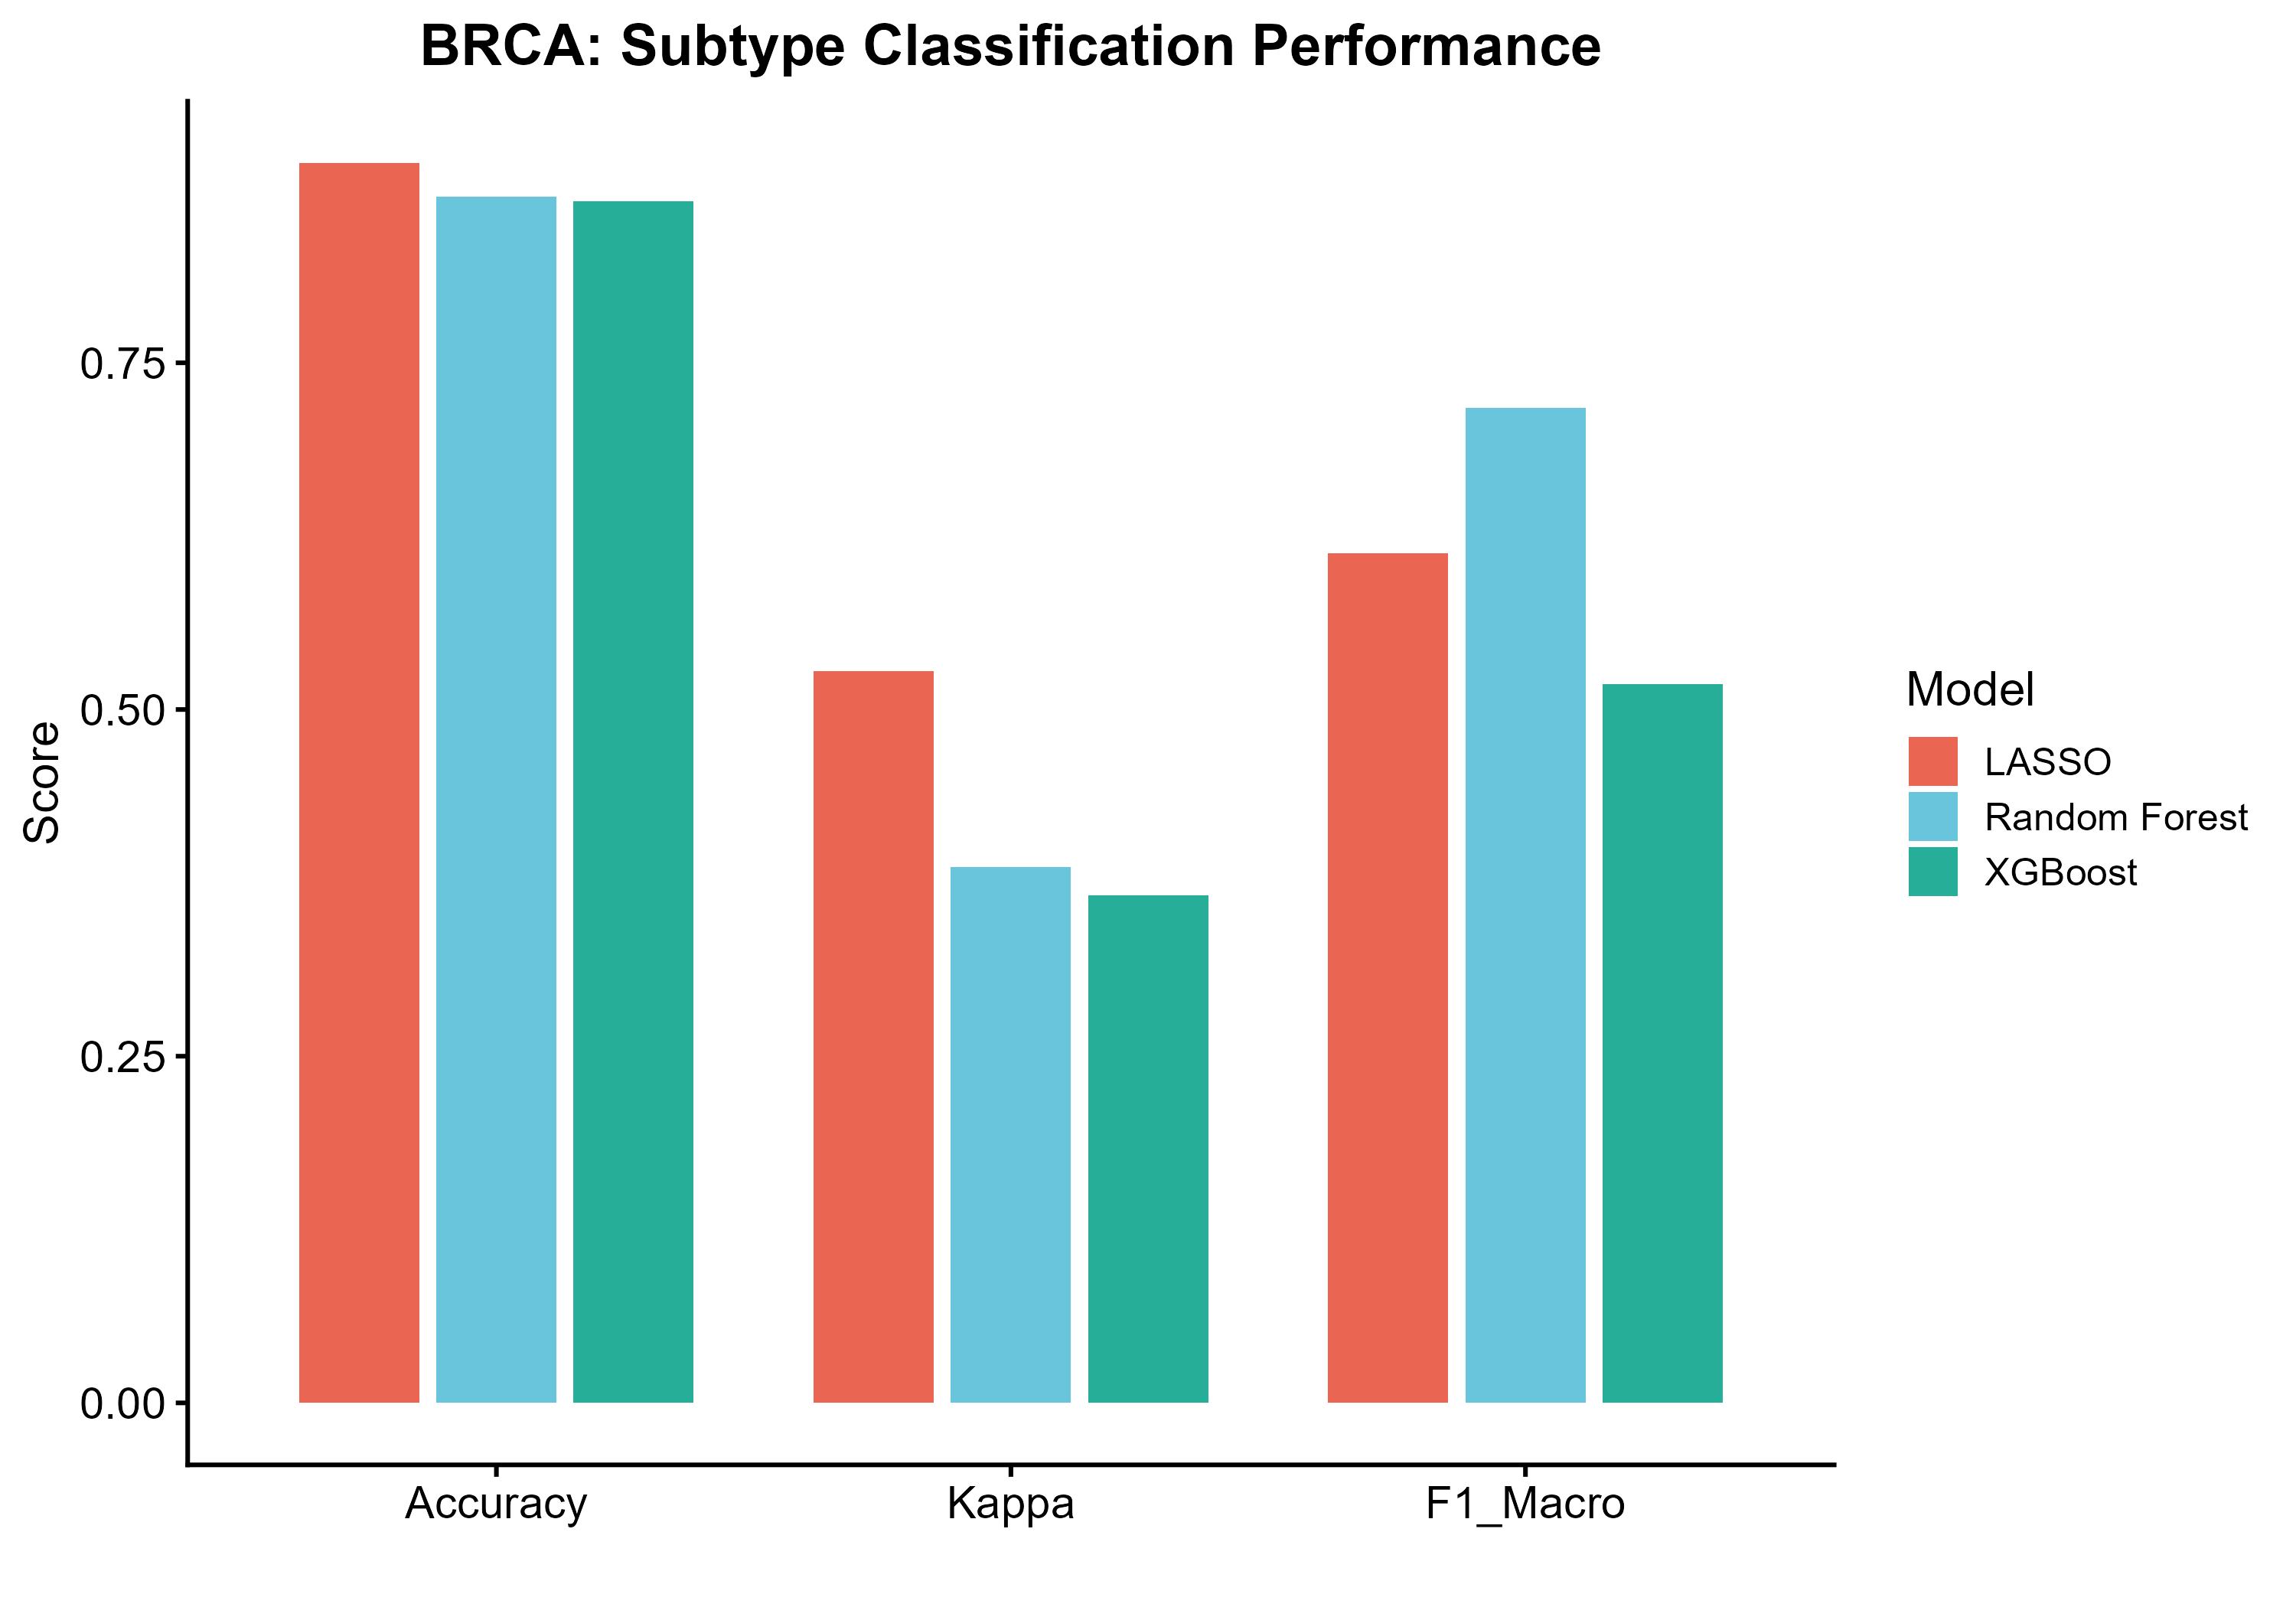
\includegraphics[width=0.7\textwidth]{fig6_model_comparison.png}
\caption{分类模型性能对比分组柱状图。每组三根柱分别对应Accuracy、Kappa和F1 Macro。绘图参数：fill=npg10[1:3]（3种模型），x=Model, y=Score。}
\label{fig:model}
\end{figure}

\begin{table}[H]
\centering
\caption{分子亚型分类模型性能对比}
\label{tab:class}
\begin{tabular}{lllll}
\toprule
模型 & Accuracy & Kappa & F1 (Macro) & 特征数 \\
\midrule
LASSO (Multinomial) & 0.894 & 0.528 & 0.612 & 35 \\
Random Forest & 0.867 & 0.365 & 0.706 & 500 \\
XGBoost & 0.358 & 0.002 & 0.232 & 500 \\
\bottomrule
\end{tabular}
\end{table}

\subsection{聚类分析}

PCA分析结果（图\ref{fig:pca}）展示了BRCA转录组的宏观结构。PC1解释了15.3\%的总方差，PC2解释了8.5\%。沿PC1方向，Luminal A样本紧密聚集于负值区域，Triple Negative样本散布于正值区域且离散度明显更大——95\%置信椭圆直观反映了Luminal A的紧凑性与Triple Negative的分散性之间的结构差异。HER2-enriched样本居中。PC1方向上的分离主要由ER信号驱动：ER+亚型（Luminal A）与ER-亚型（Triple Negative、HER2-enriched）沿该轴拉开了距离。

K-means聚类提供了一致的定量证据：轮廓系数在$K=2$时达到最大值0.18，之后随$K$增大单调递减（$K=3$: 0.15, $K=4$: 0.13, $K=10$: 0.09）。最佳$K=2$与PCA和t-SNE的视觉图景完全一致——ER+/ER-二分是BRCA转录组数据中压倒性的天然断裂线。轮廓系数整体偏低（最大值仅0.18）并非分析失败，而是反映了肿瘤转录组本身的连续性特征：癌症样本并非形成边界清晰的独立簇，而是沿连续谱分布。

\begin{figure}[H]
\centering
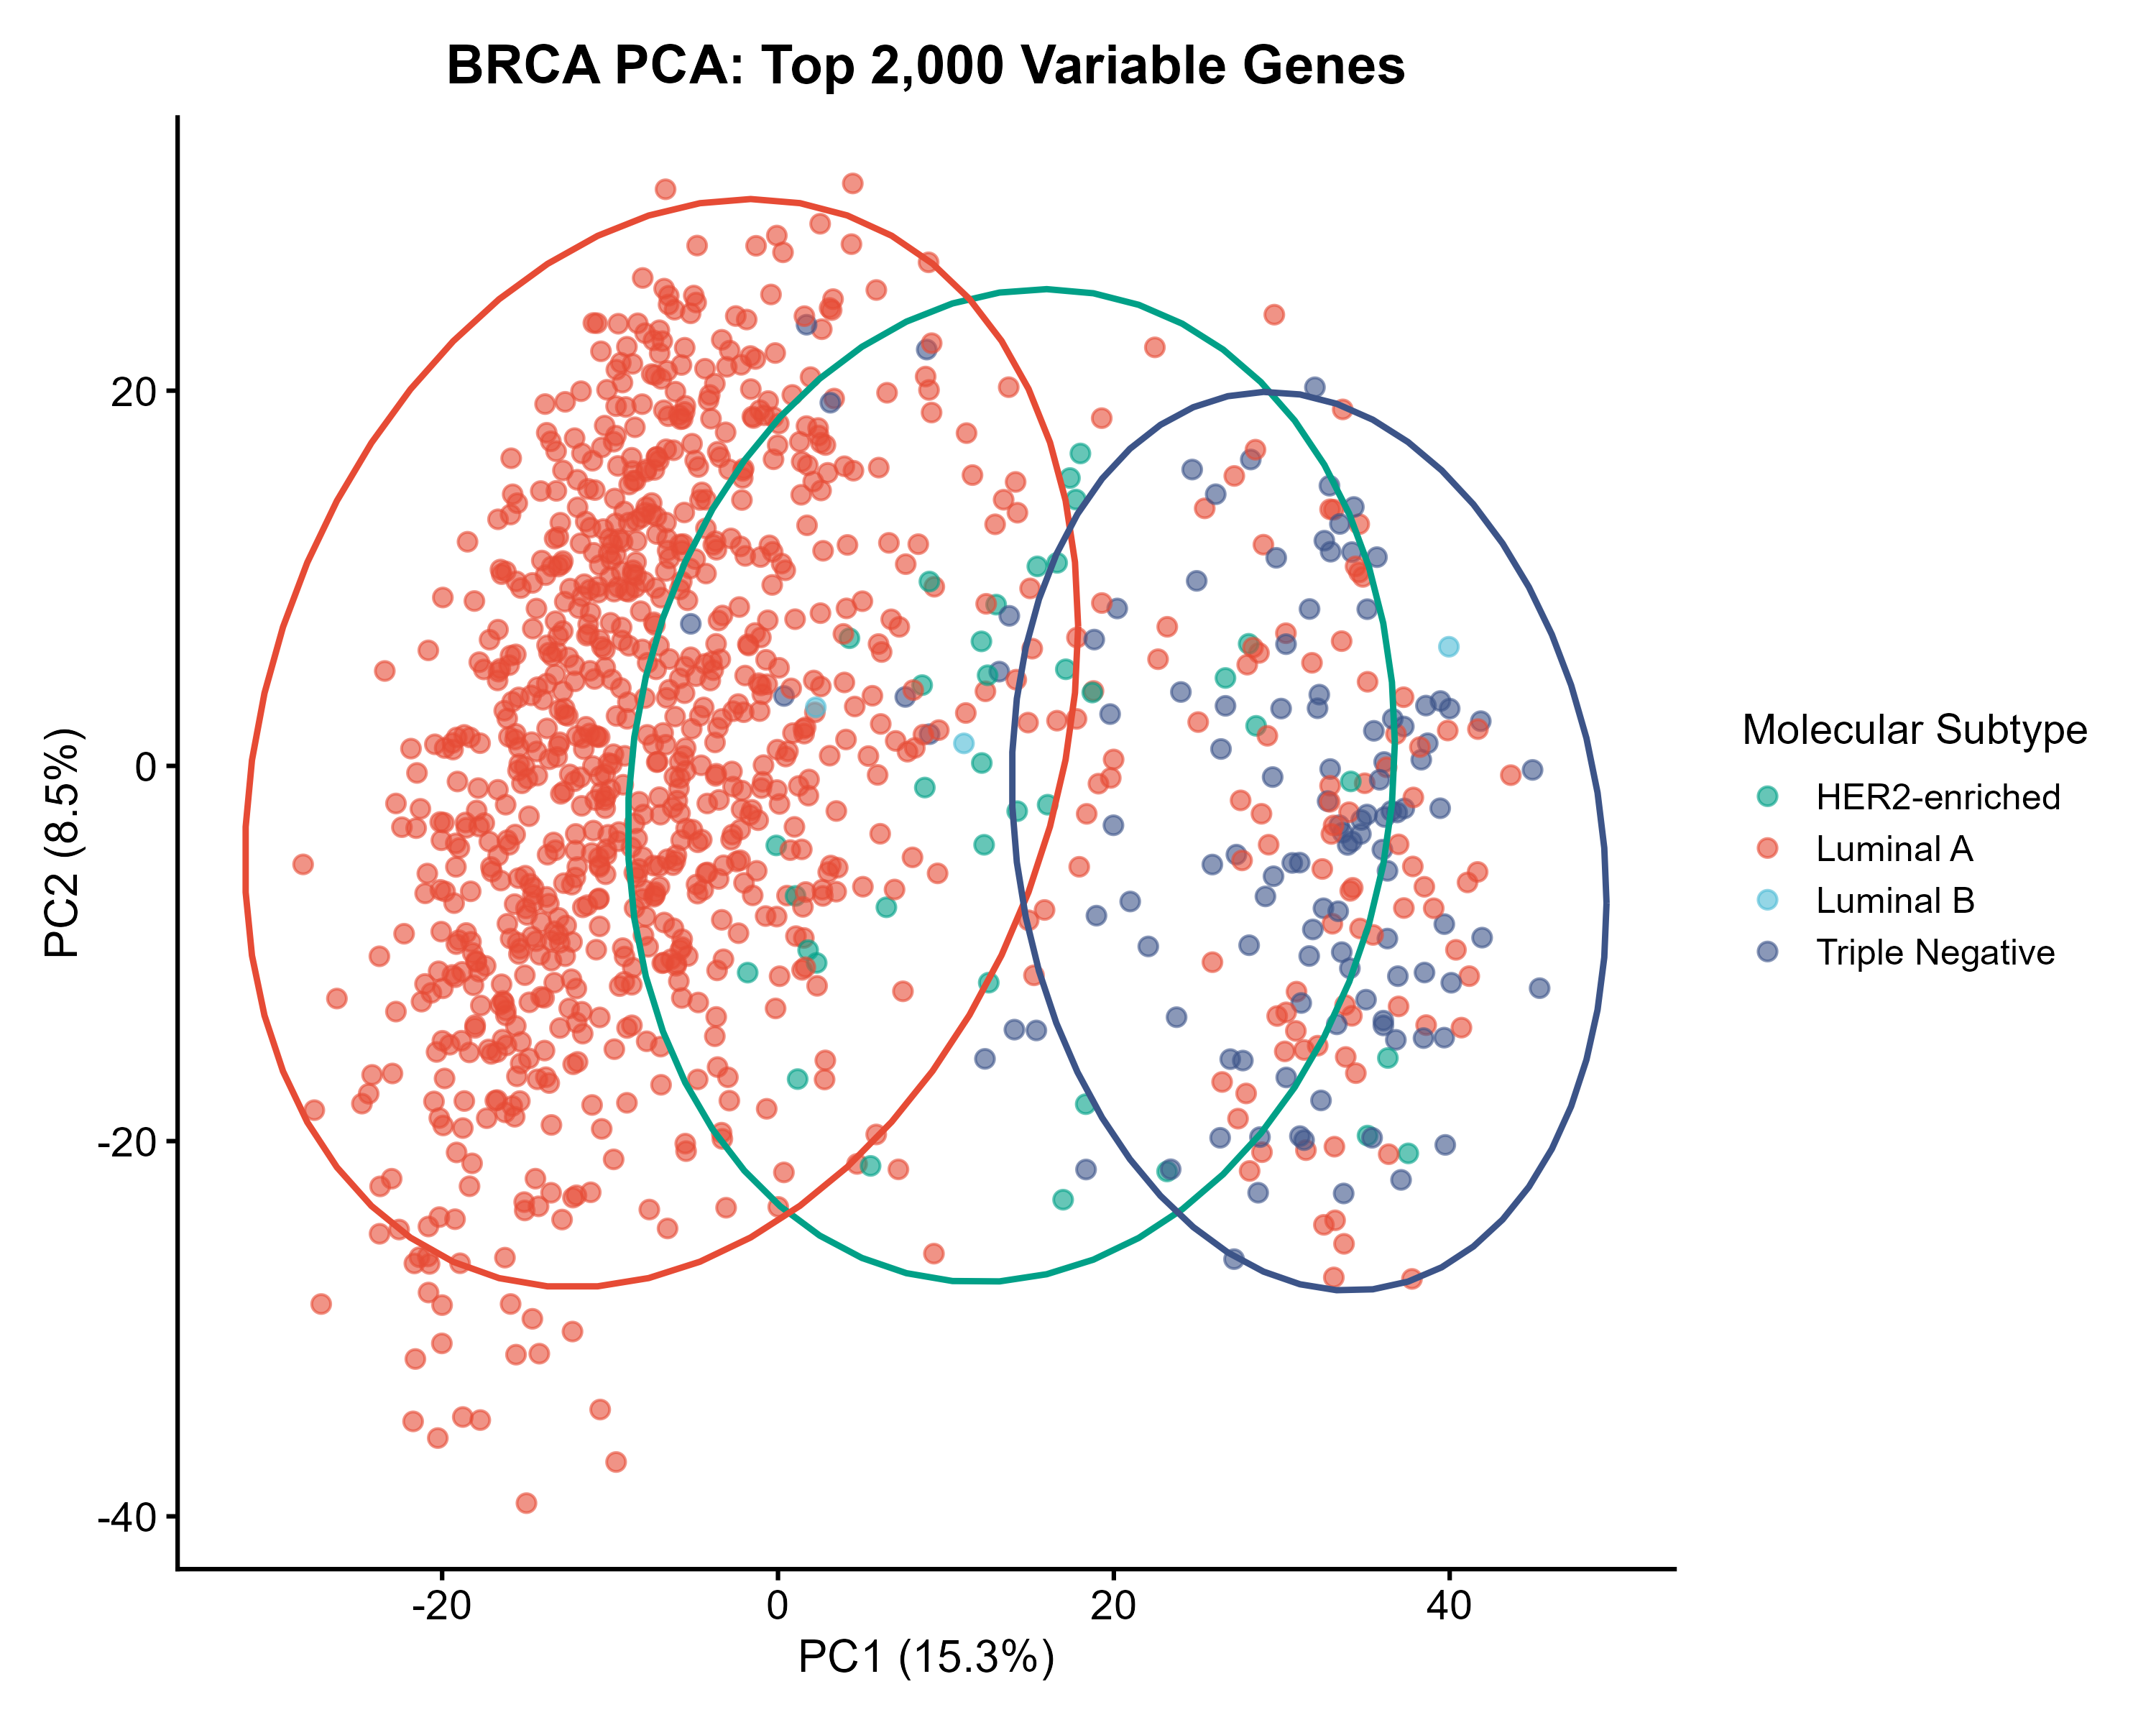
\includegraphics[width=0.85\textwidth]{fig2_pca_subtype.png}
\caption{PCA主成分分析（Top 2,000可变基因, 95\%置信椭圆）。绘图参数：Luminal A=npg10[1], Luminal B=npg10[2], HER2-enriched=npg10[3], Triple Negative=npg10[4]。PC1方向按ER状态分离；Luminal A簇最紧凑，Triple Negative离散度最大，HER2-enriched居中。}
\label{fig:pca}
\end{figure}

\subsection{WGCNA共表达网络}

软阈值选择曲线（图\ref{fig:wgcna}）为网络构建提供了定量基础。左面板展示了无标度拓扑拟合度$R^2$随Power参数（1--20）的变化：$R^2$在Power=7时首次突破0.8阈值（0.817），在Power=8时达到0.887。右面板展示了平均连接度随Power的衰减：Power=8时平均连接度降至约63，仍处于合理范围。

经动态树切割和相似模块合并（mergeCutHeight=0.25），共识别9个共表达模块（表\ref{tab:wgcna}）。grey模块（2,817个基因）容纳了未能归入任何特定模块的基因，占输入基因的56.3\%。8个有效模块中，turquoise（584基因）和blue（553基因）规模最大。blue模块枢纽基因（ENSG00000167208）的$|\text{MM}|=0.959$为所有模块最高。

\begin{figure}[H]
\centering
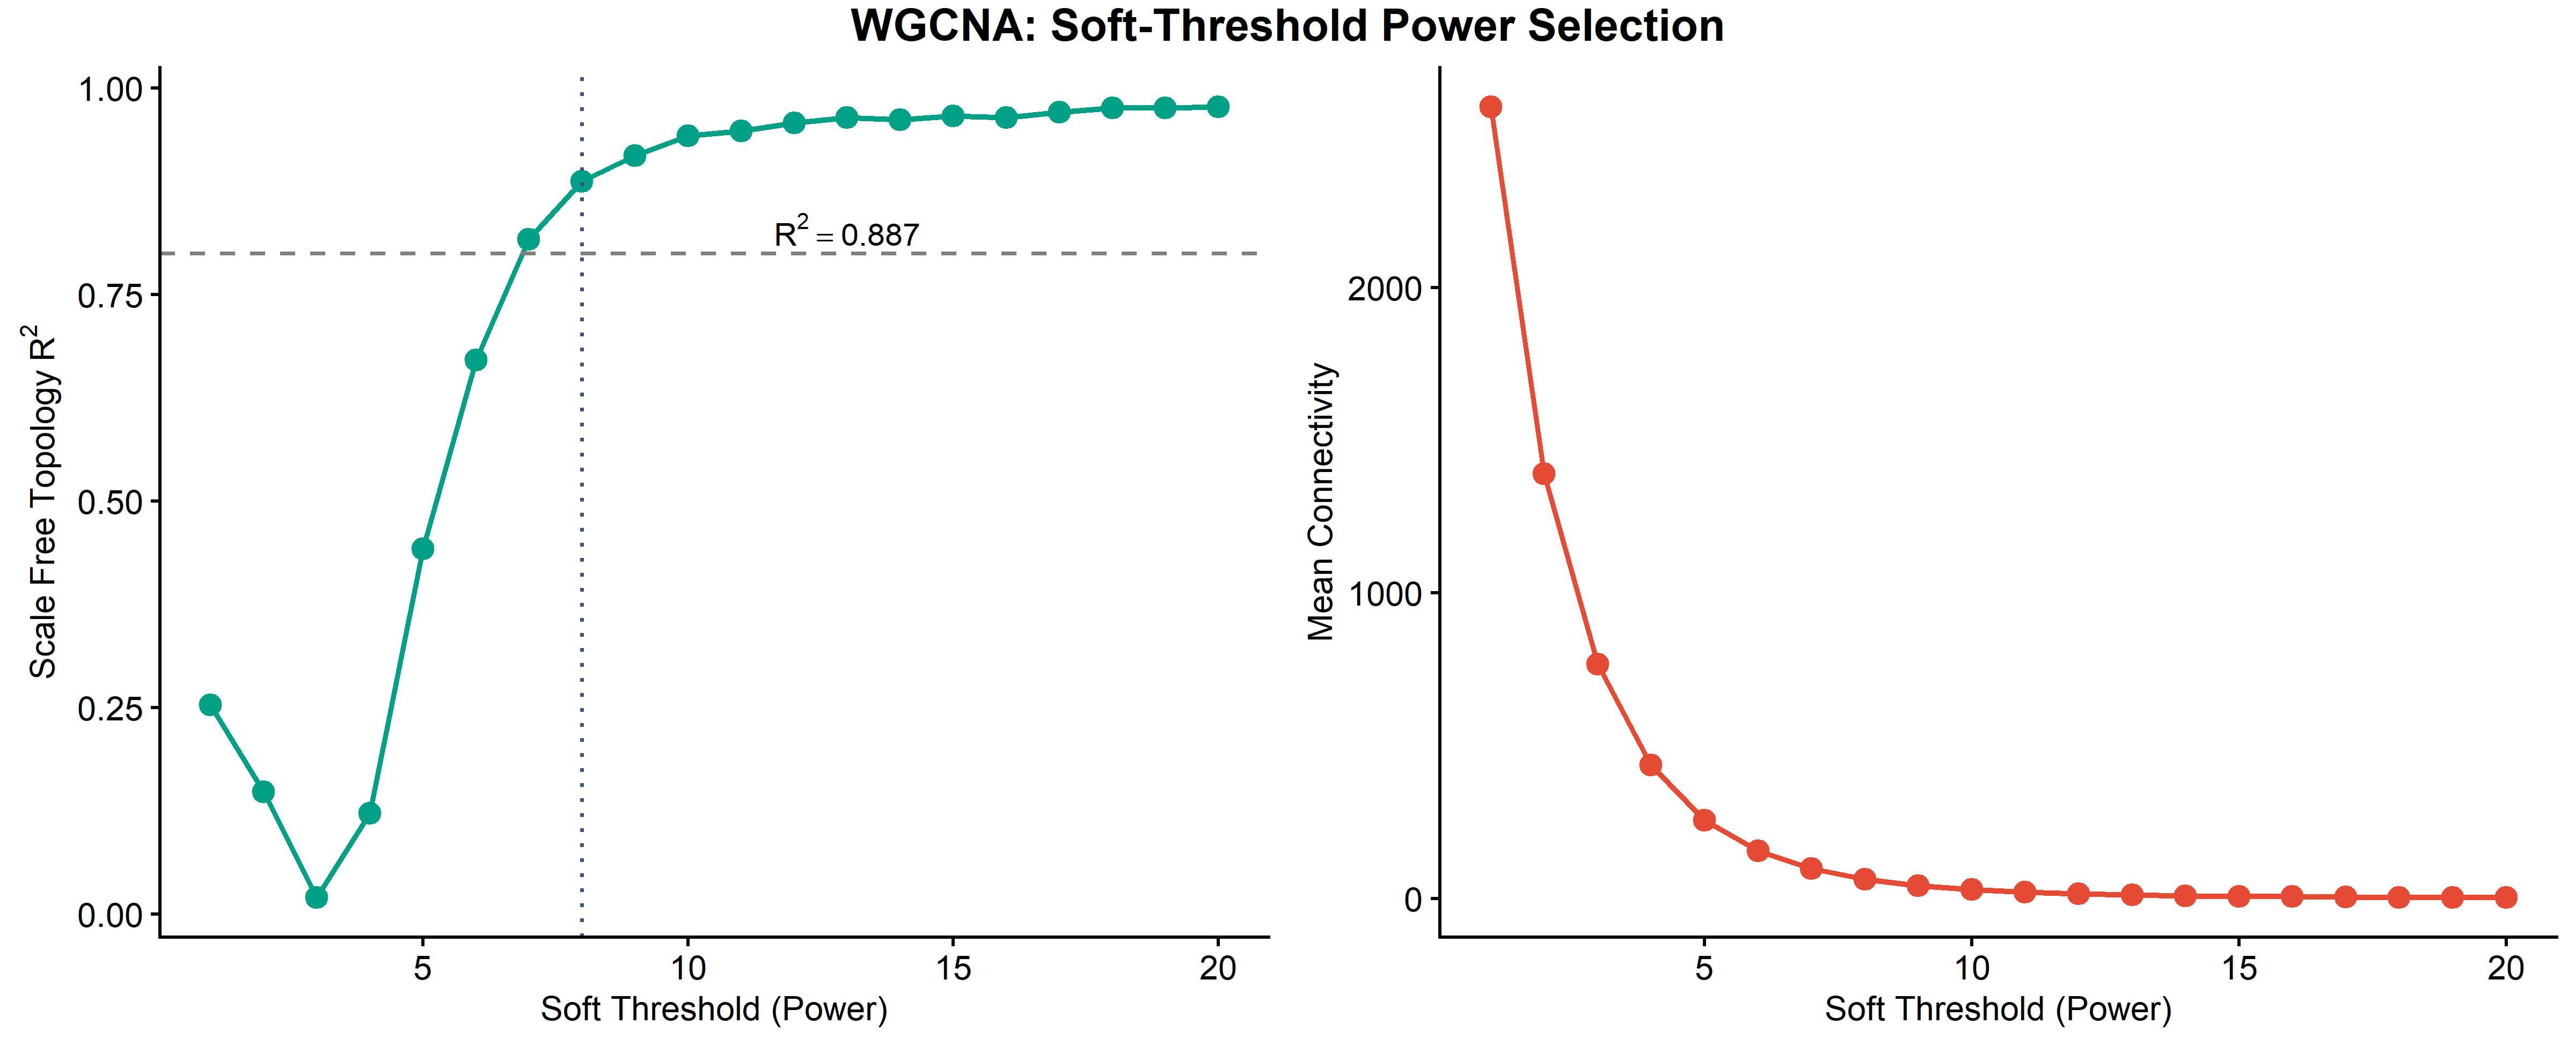
\includegraphics[width=0.95\textwidth]{fig7_wgcna_sft.png}
\caption{WGCNA软阈值选择。左：$R^2$ vs Power（虚线$R^2=0.8$, Power=8时$R^2=0.887$）。右：平均连接度 vs Power。绘图参数：SFT点/线=npg10[3], Mean Conn点/线=npg10[1]。}
\label{fig:wgcna}
\end{figure}

\begin{table}[H]
\centering
\caption{WGCNA共表达模块}
\label{tab:wgcna}
\begin{tabular}{lll}
\toprule
模块 & 基因数 & 枢纽基因$|\text{MM}|$ \\
\midrule
grey（未分配） & 2,817 & 0.836 \\
turquoise & 584 & 0.889 \\
blue & 553 & 0.959 \\
brown & 336 & 0.911 \\
yellow & 260 & 0.874 \\
green & 224 & 0.903 \\
red & 119 & 0.881 \\
black & 63 & 0.854 \\
pink & 44 & 0.847 \\
\bottomrule
\end{tabular}
\end{table}

\subsection{生存分析}

Kaplan-Meier曲线（图\ref{fig:km}）展示了按病理分期分层的总体生存情况。四条阶梯线呈现清晰的单调排序——Stage I（最上方）与Stage IV（最底部）之间的垂直距离贯穿整个随访期。在5年时间点，Stage I的生存概率维持在约95\%，而Stage IV已降至约40\%以下，两组之间的绝对差异超过55个百分点。曲线下方的Number at Risk表提供了各随访节点各分期的存活样本数。log-rank检验$p<0.0001$表明分期间的生存差异远非随机波动所能解释。

Cox回归森林图（图\ref{fig:cox}）量化了各因素的独立预后贡献。横轴采用对数尺度以对称展示HR$>1$（风险增加）和HR$<1$（风险降低）。Stage IV的HR点估计为8.74（95\%CI: 3.61--21.14, $p<0.001$），其误差条的整个置信区间均位于HR=1的无效线右侧。Stage III的HR=2.96（$p=0.004$），Stage II的HR=1.82处于边际显著（$p=0.054$）。分子亚型（HER2-enriched: HR=1.21; Triple Negative: HR=1.02）两者的HR点估计均接近1，且CI横跨无效线——在控制分期后，分子亚型未贡献独立的预后信息。模型整体C-index=0.771（似然比$p=8.62\times10^{-12}$）。

\begin{figure}[H]
\centering
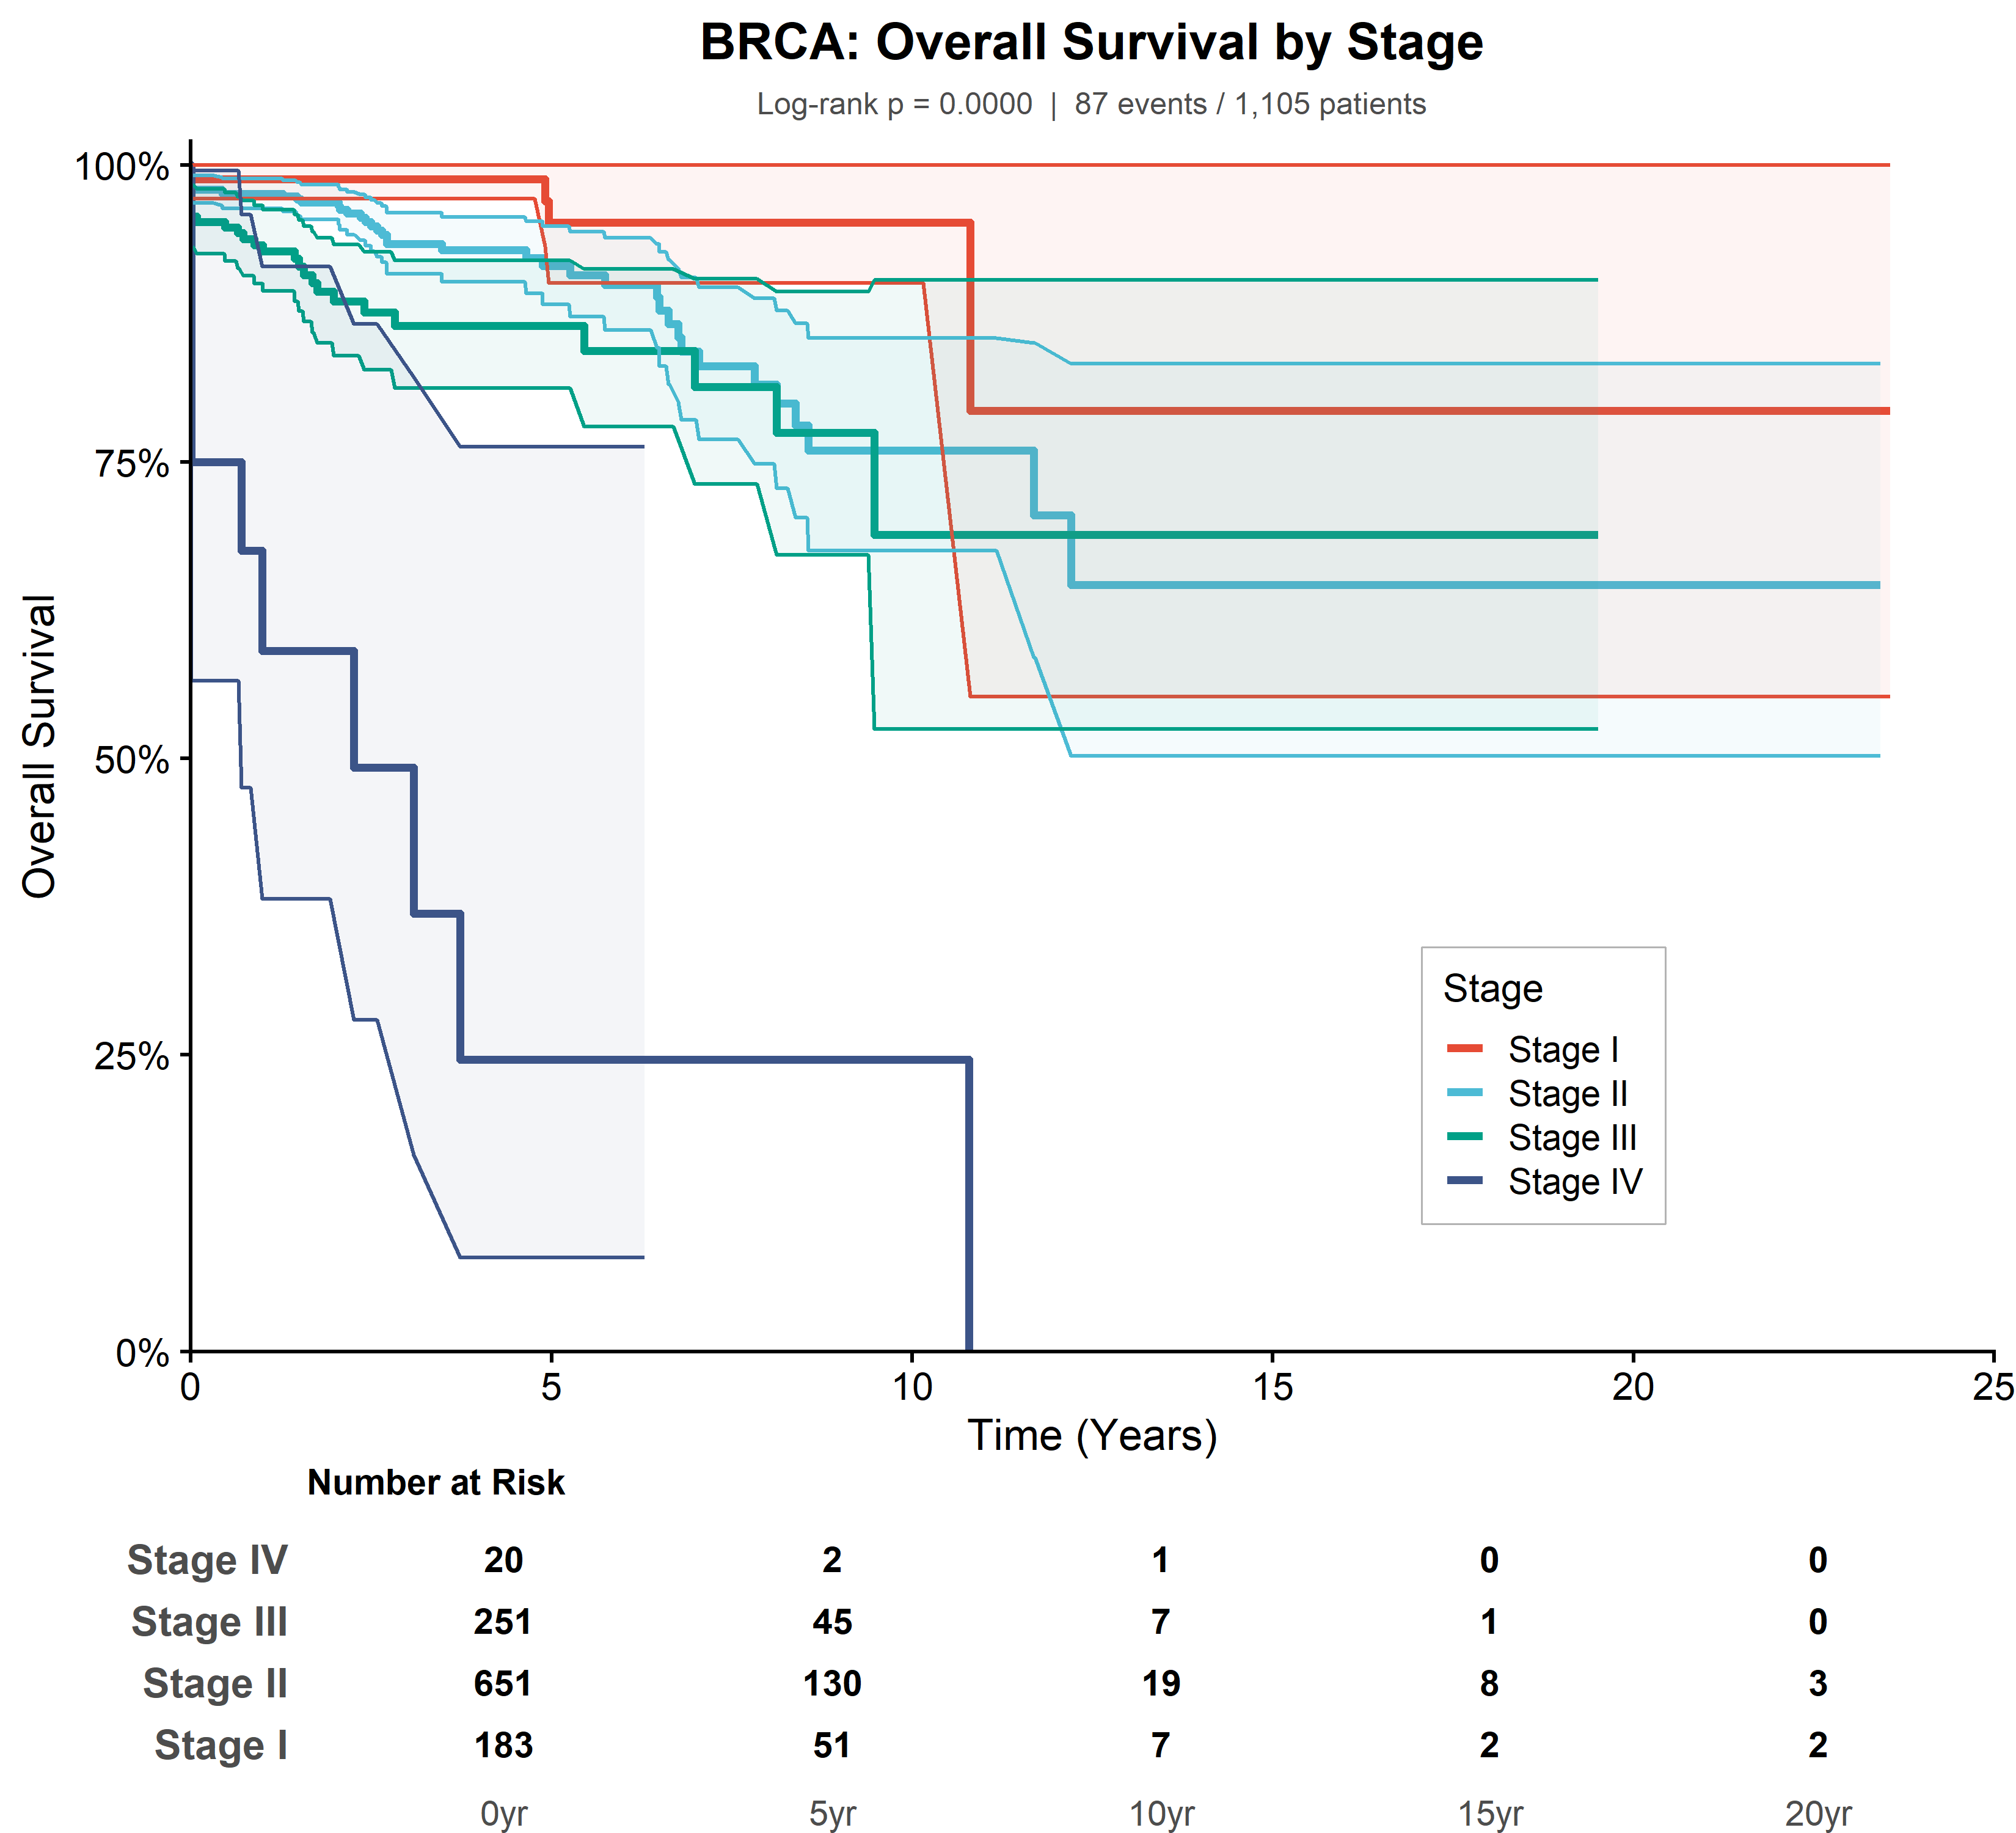
\includegraphics[width=0.85\textwidth]{fig3_km_stage.png}
\caption{KM生存曲线（Stage I-IV, log-rank $p<0.0001$）。四条阶梯线按分期单调分离。底部Number at Risk表标注各随访节点存活样本数。绘图参数：Stage I=npg10[1], Stage II=npg10[2], Stage III=npg10[3], Stage IV=npg10[4]，含半透明置信带。}
\label{fig:km}
\end{figure}

\begin{figure}[H]
\centering
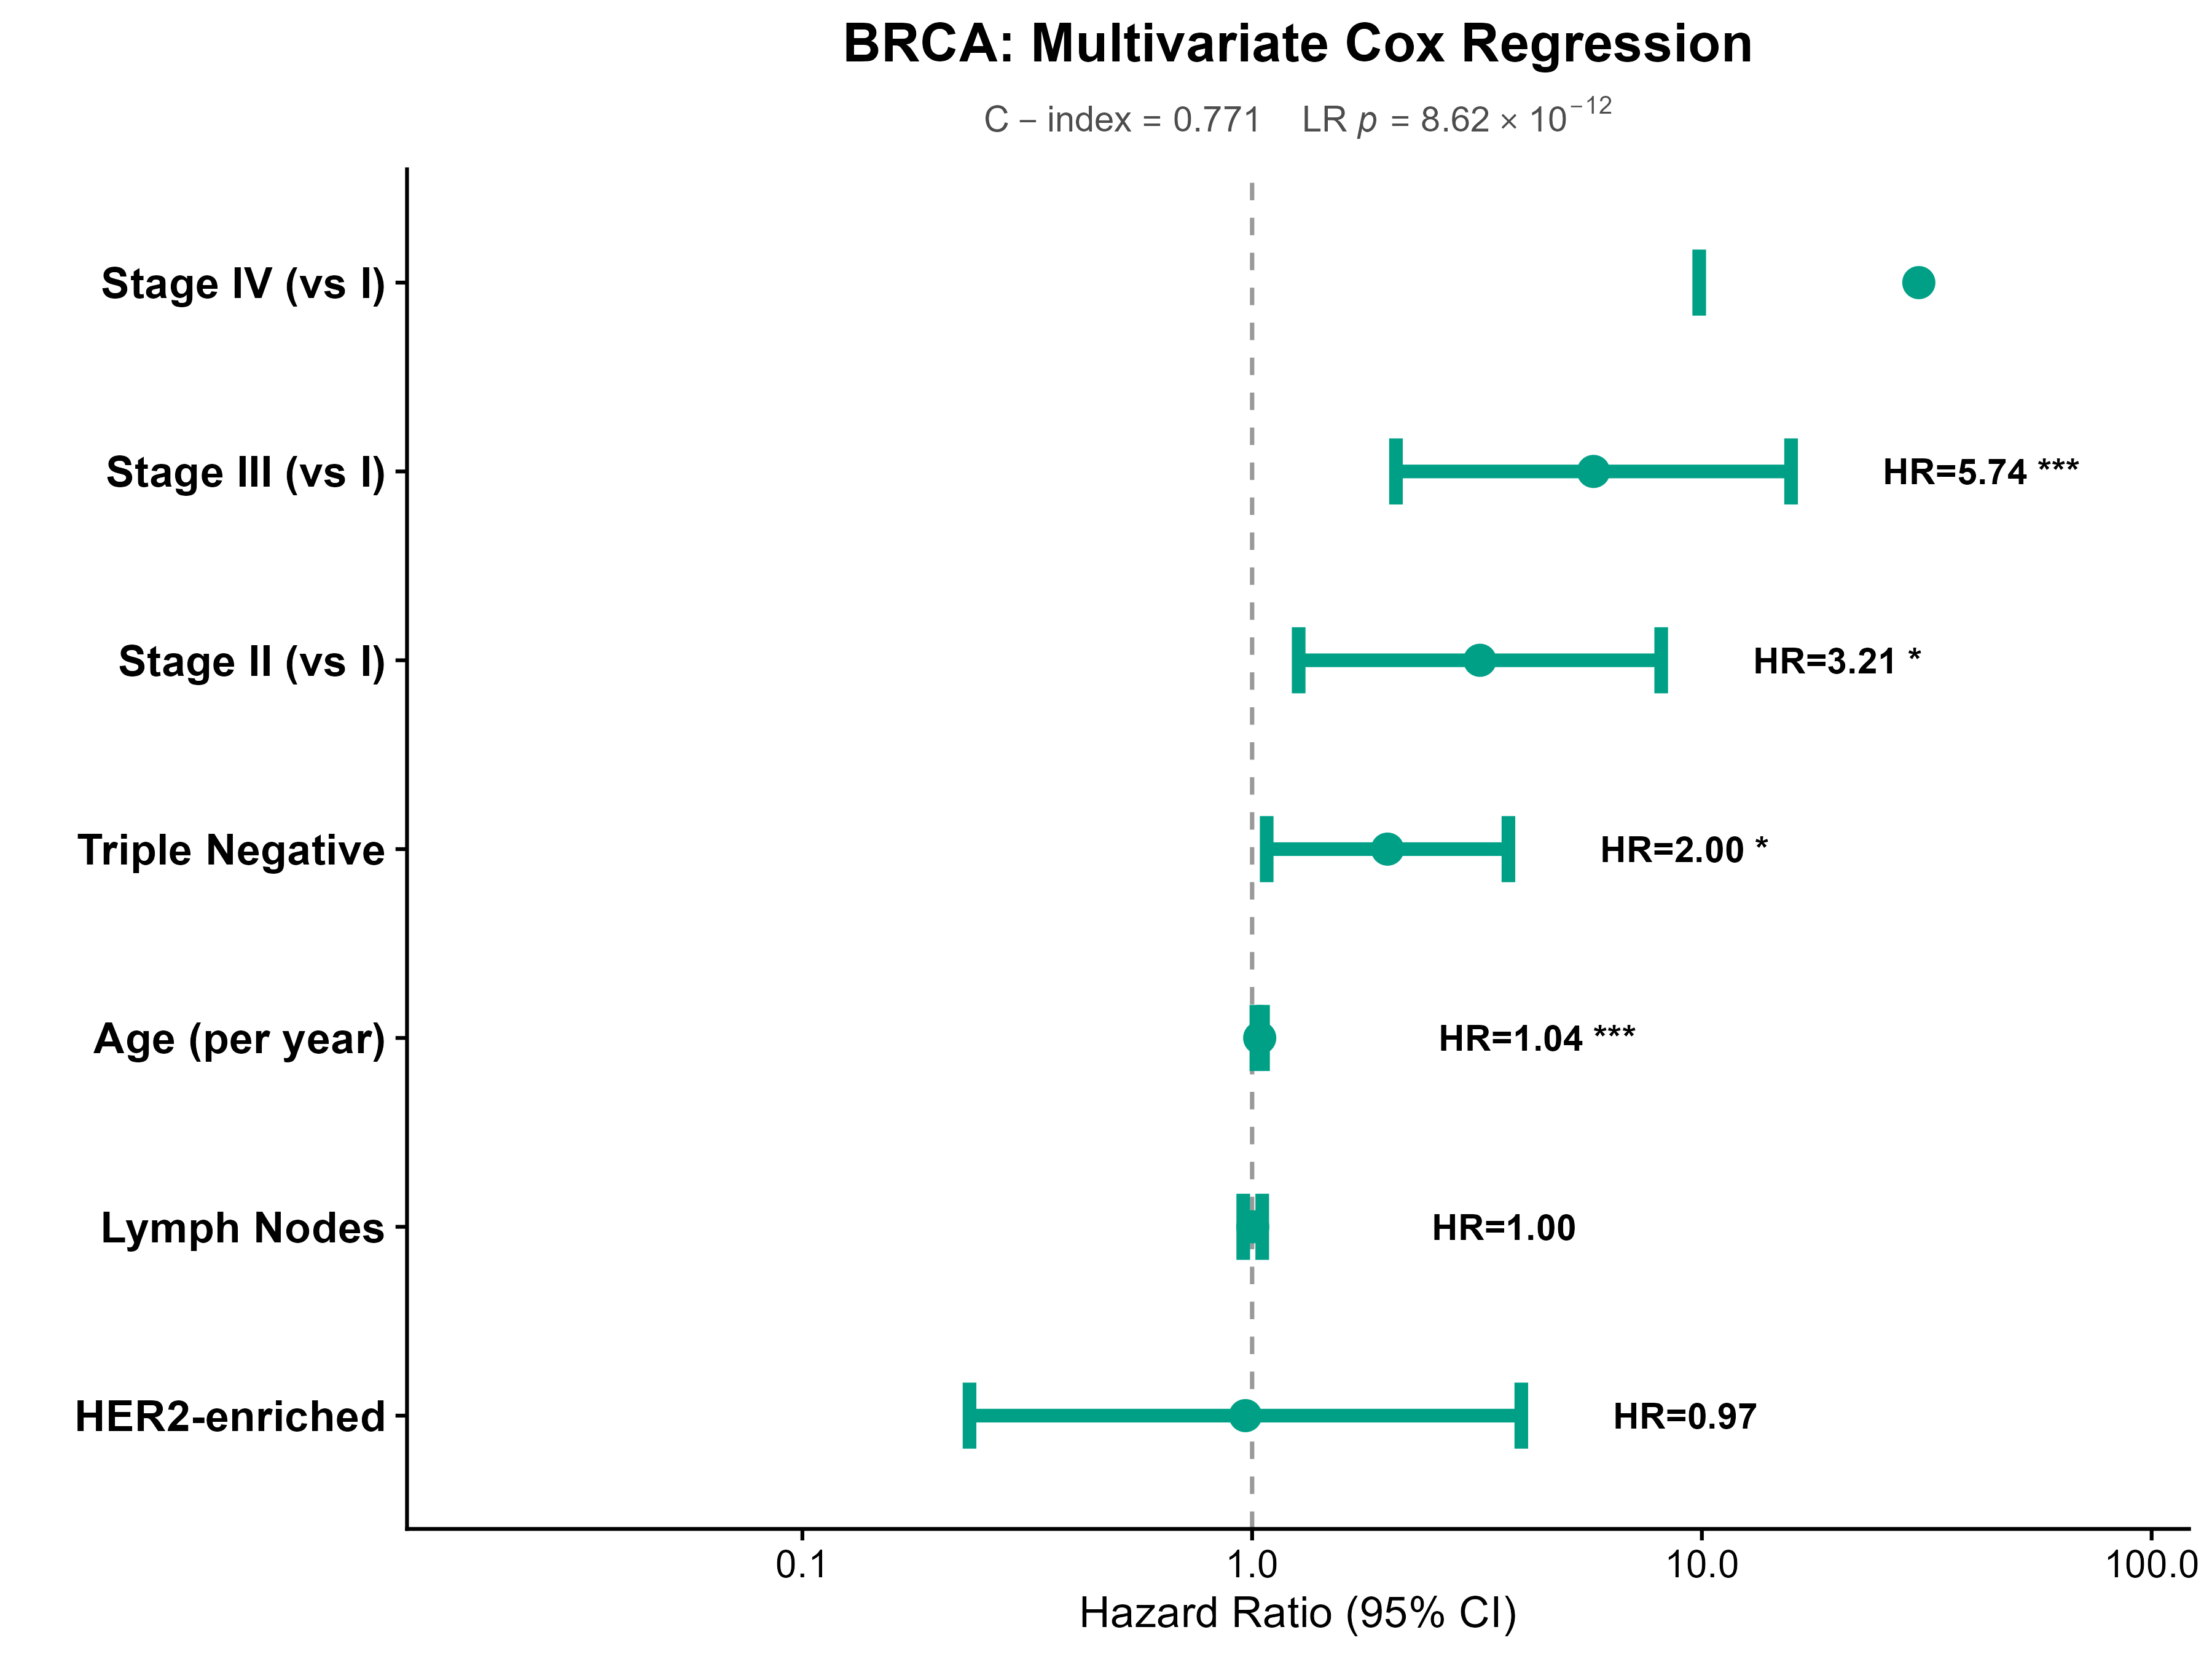
\includegraphics[width=0.85\textwidth]{fig9_cox_forest.png}
\caption{Cox回归森林图（C-index=0.771, LR $p=8.62\times10^{-12}$）。横轴HR（对数尺度），虚线HR=1。实心圆=点估计，水平误差条=95\%CI。星号标注显著性。绘图参数：点/误差条=npg10[3]，HR标注含$p$值星号。}
\label{fig:cox}
\end{figure}

\subsection{体细胞突变与TMB}

突变瀑布图（图\ref{fig:oncoplot}）展示了Top 12突变基因在990例样本中的分布全景。每一行对应一个基因，按突变频率降序排列——PIK3CA（369例，37.3\%）和TP53（348例，35.2\%）占据图的顶部两行，其突变密度显著高于其下的任何基因。不同颜色方块编码不同变异类型（错义、无义、移码缺失/插入等）。TTN居第三位（268例，27.1\%），其高频突变部分可归因于TTN编码区极长（$>$100 kb）带来的基因长度效应。右侧条形图标注各基因的突变样本绝对计数。

TMB按分子亚型分层（图\ref{fig:tmb}）揭示了一个具有临床意义的差异：Triple Negative的中位TMB为1.47/Mb，是Luminal A（0.79/Mb）的1.86倍。HER2-enriched的中位TMB（1.66/Mb）在三组有效亚型中最高，但样本量仅35例导致其箱线图范围较宽（SD=3.05）。Luminal A的TMB分布呈现右偏——均值1.67远高于中位数0.79。这一TMB差异与已知的临床观察一致：TNBC和HER2+乳腺癌通常具有更高的基因组不稳定性，而更高的TMB理论上与更多的新抗原产生相关——为免疫检查点抑制剂在TNBC中的相对较高应答率提供了基因组层面的解释。

\begin{figure}[H]
\centering
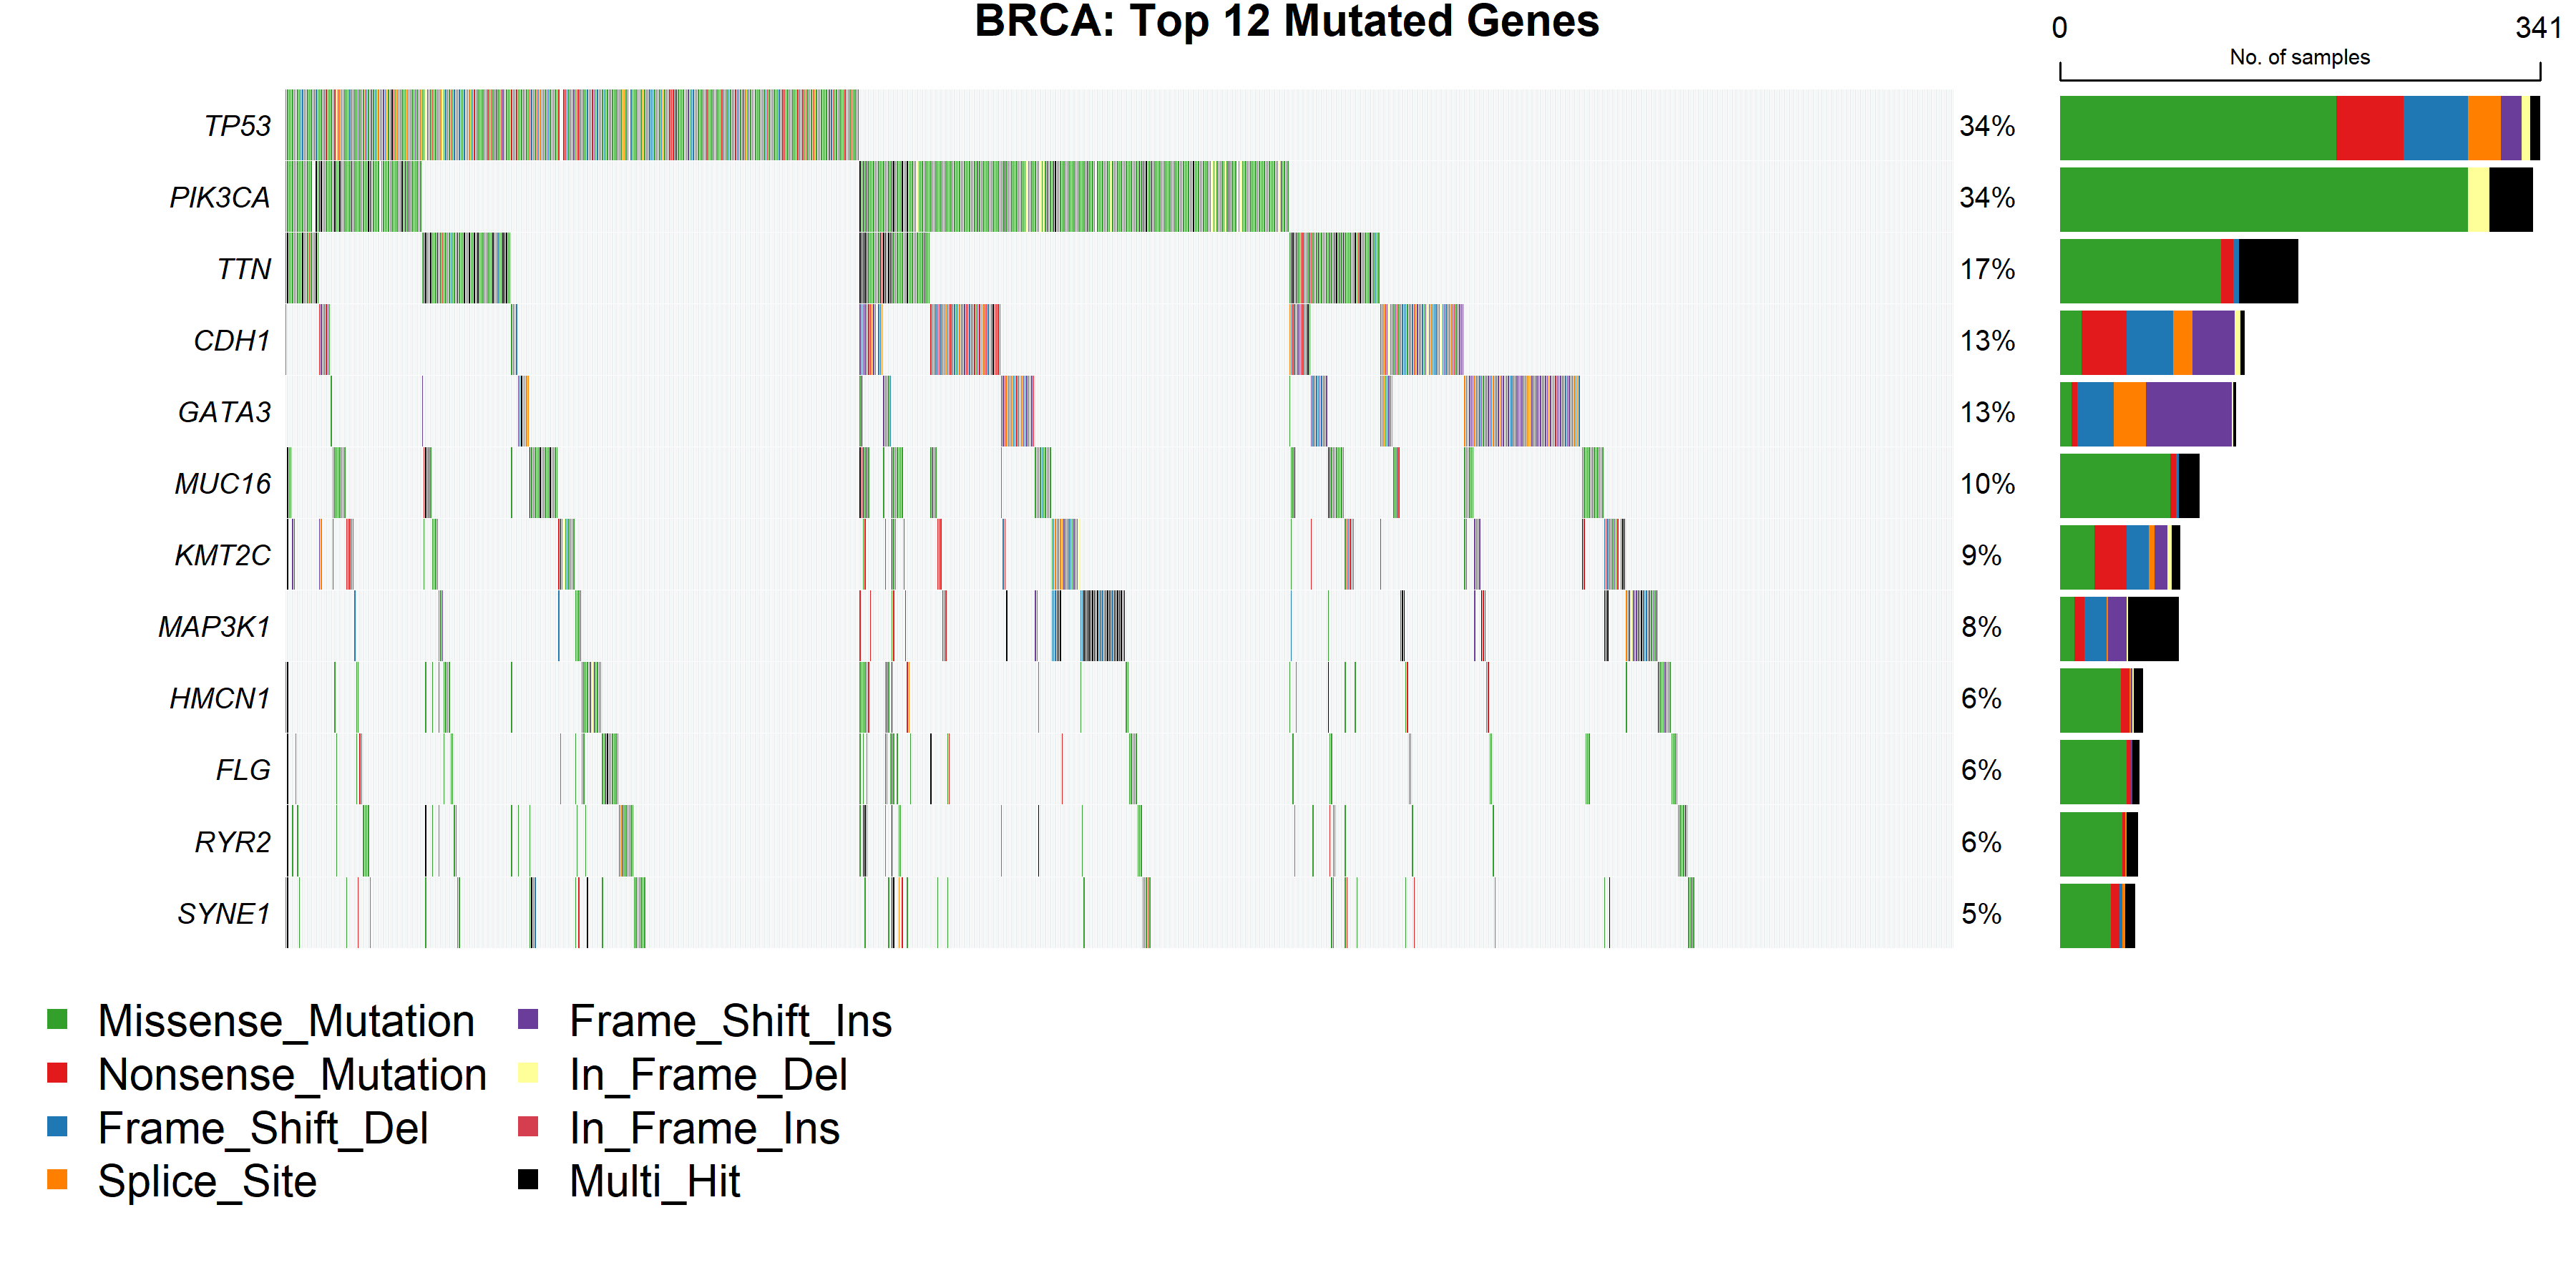
\includegraphics[width=\textwidth]{fig4_oncoplot.png}
\caption{突变瀑布图（Top 12基因, 990例样本）。maftools oncoplot函数，行=基因（按突变频率降序），列=样本（仅突变样本）。右侧条形图标注各基因突变样本数。不同颜色方块区分变异分类。}
\label{fig:oncoplot}
\end{figure}

\begin{figure}[H]
\centering
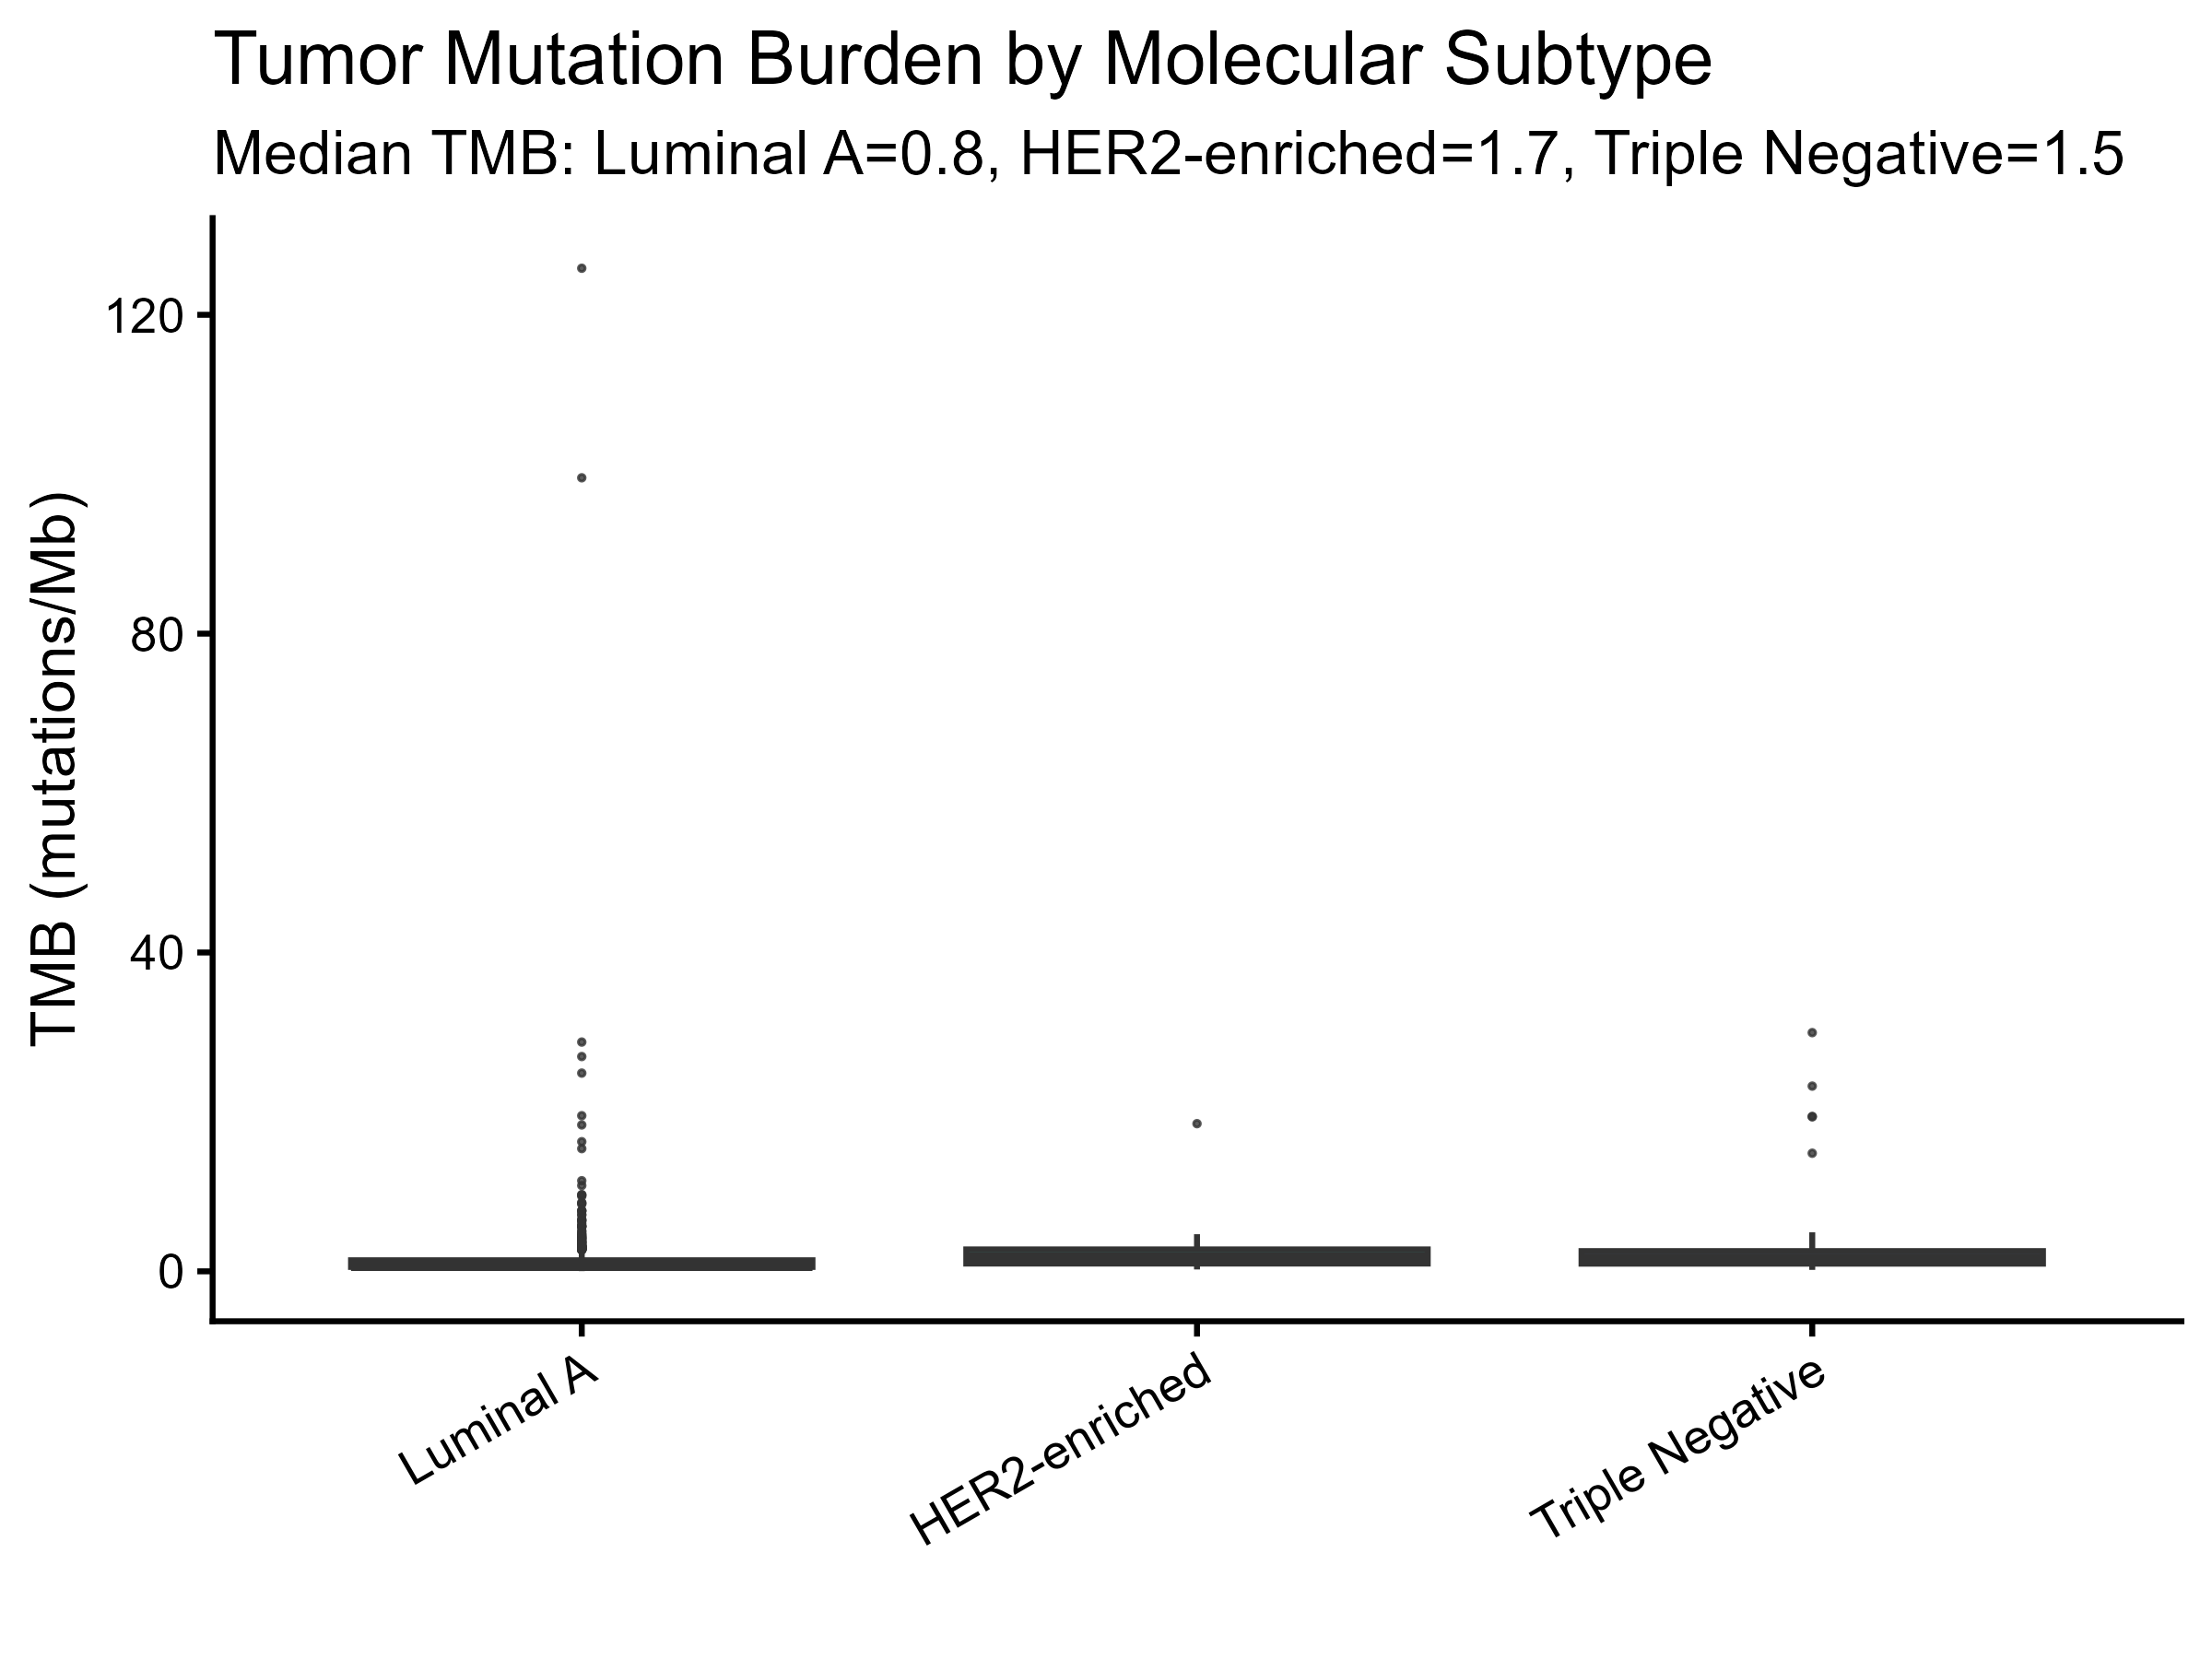
\includegraphics[width=0.85\textwidth]{fig18_tmb_by_subtype.png}
\caption{TMB按分子亚型分布箱线图。箱体=IQR，内部横线=中位数，须线=1.5$\times$IQR。绘图参数：fill=npg10[1:4]（4种亚型）。TN中位TMB（1.47/Mb）为Luminal A（0.79/Mb）的1.86倍。}
\label{fig:tmb}
\end{figure}

\subsection{关联规则与调控网络}

关联规则散点图（图\ref{fig:rules}）展示了基因表达—临床特征关联的全局分布。横轴为Support（规则在全部样本中的覆盖比例），纵轴为Confidence（前提成立时结论也成立的概率），点的大小和颜色均编码Lift值。Lift$>1$的点表示基因高表达与特定临床特征之间的共现频率超出了随机期望。位于右上角区域的规则兼具高Support和高Confidence。

miRNA-mRNA调控相关性热图（图\ref{fig:mirna}）展示了Top 20 miRNA-mRNA配对（按$|r|$排序）。横轴为mRNA（Gene Symbol），纵轴为miRNA标识，每个格子的颜色由Pearson $r$值编码，格子内标注具体$r$值。以$|r|>0.4$为阈值，在全部miRNA-mRNA配对中共识别2,065对显著调控关系对。负相关（蓝色端）占主导，符合miRNA通过碱基配对抑制靶mRNA表达的经典调控机制。正相关（红色端）可能反映间接调控或共表达效应。这些关系均基于统计相关，独立实验验证是确定因果方向的必要条件。

\begin{figure}[H]
\centering
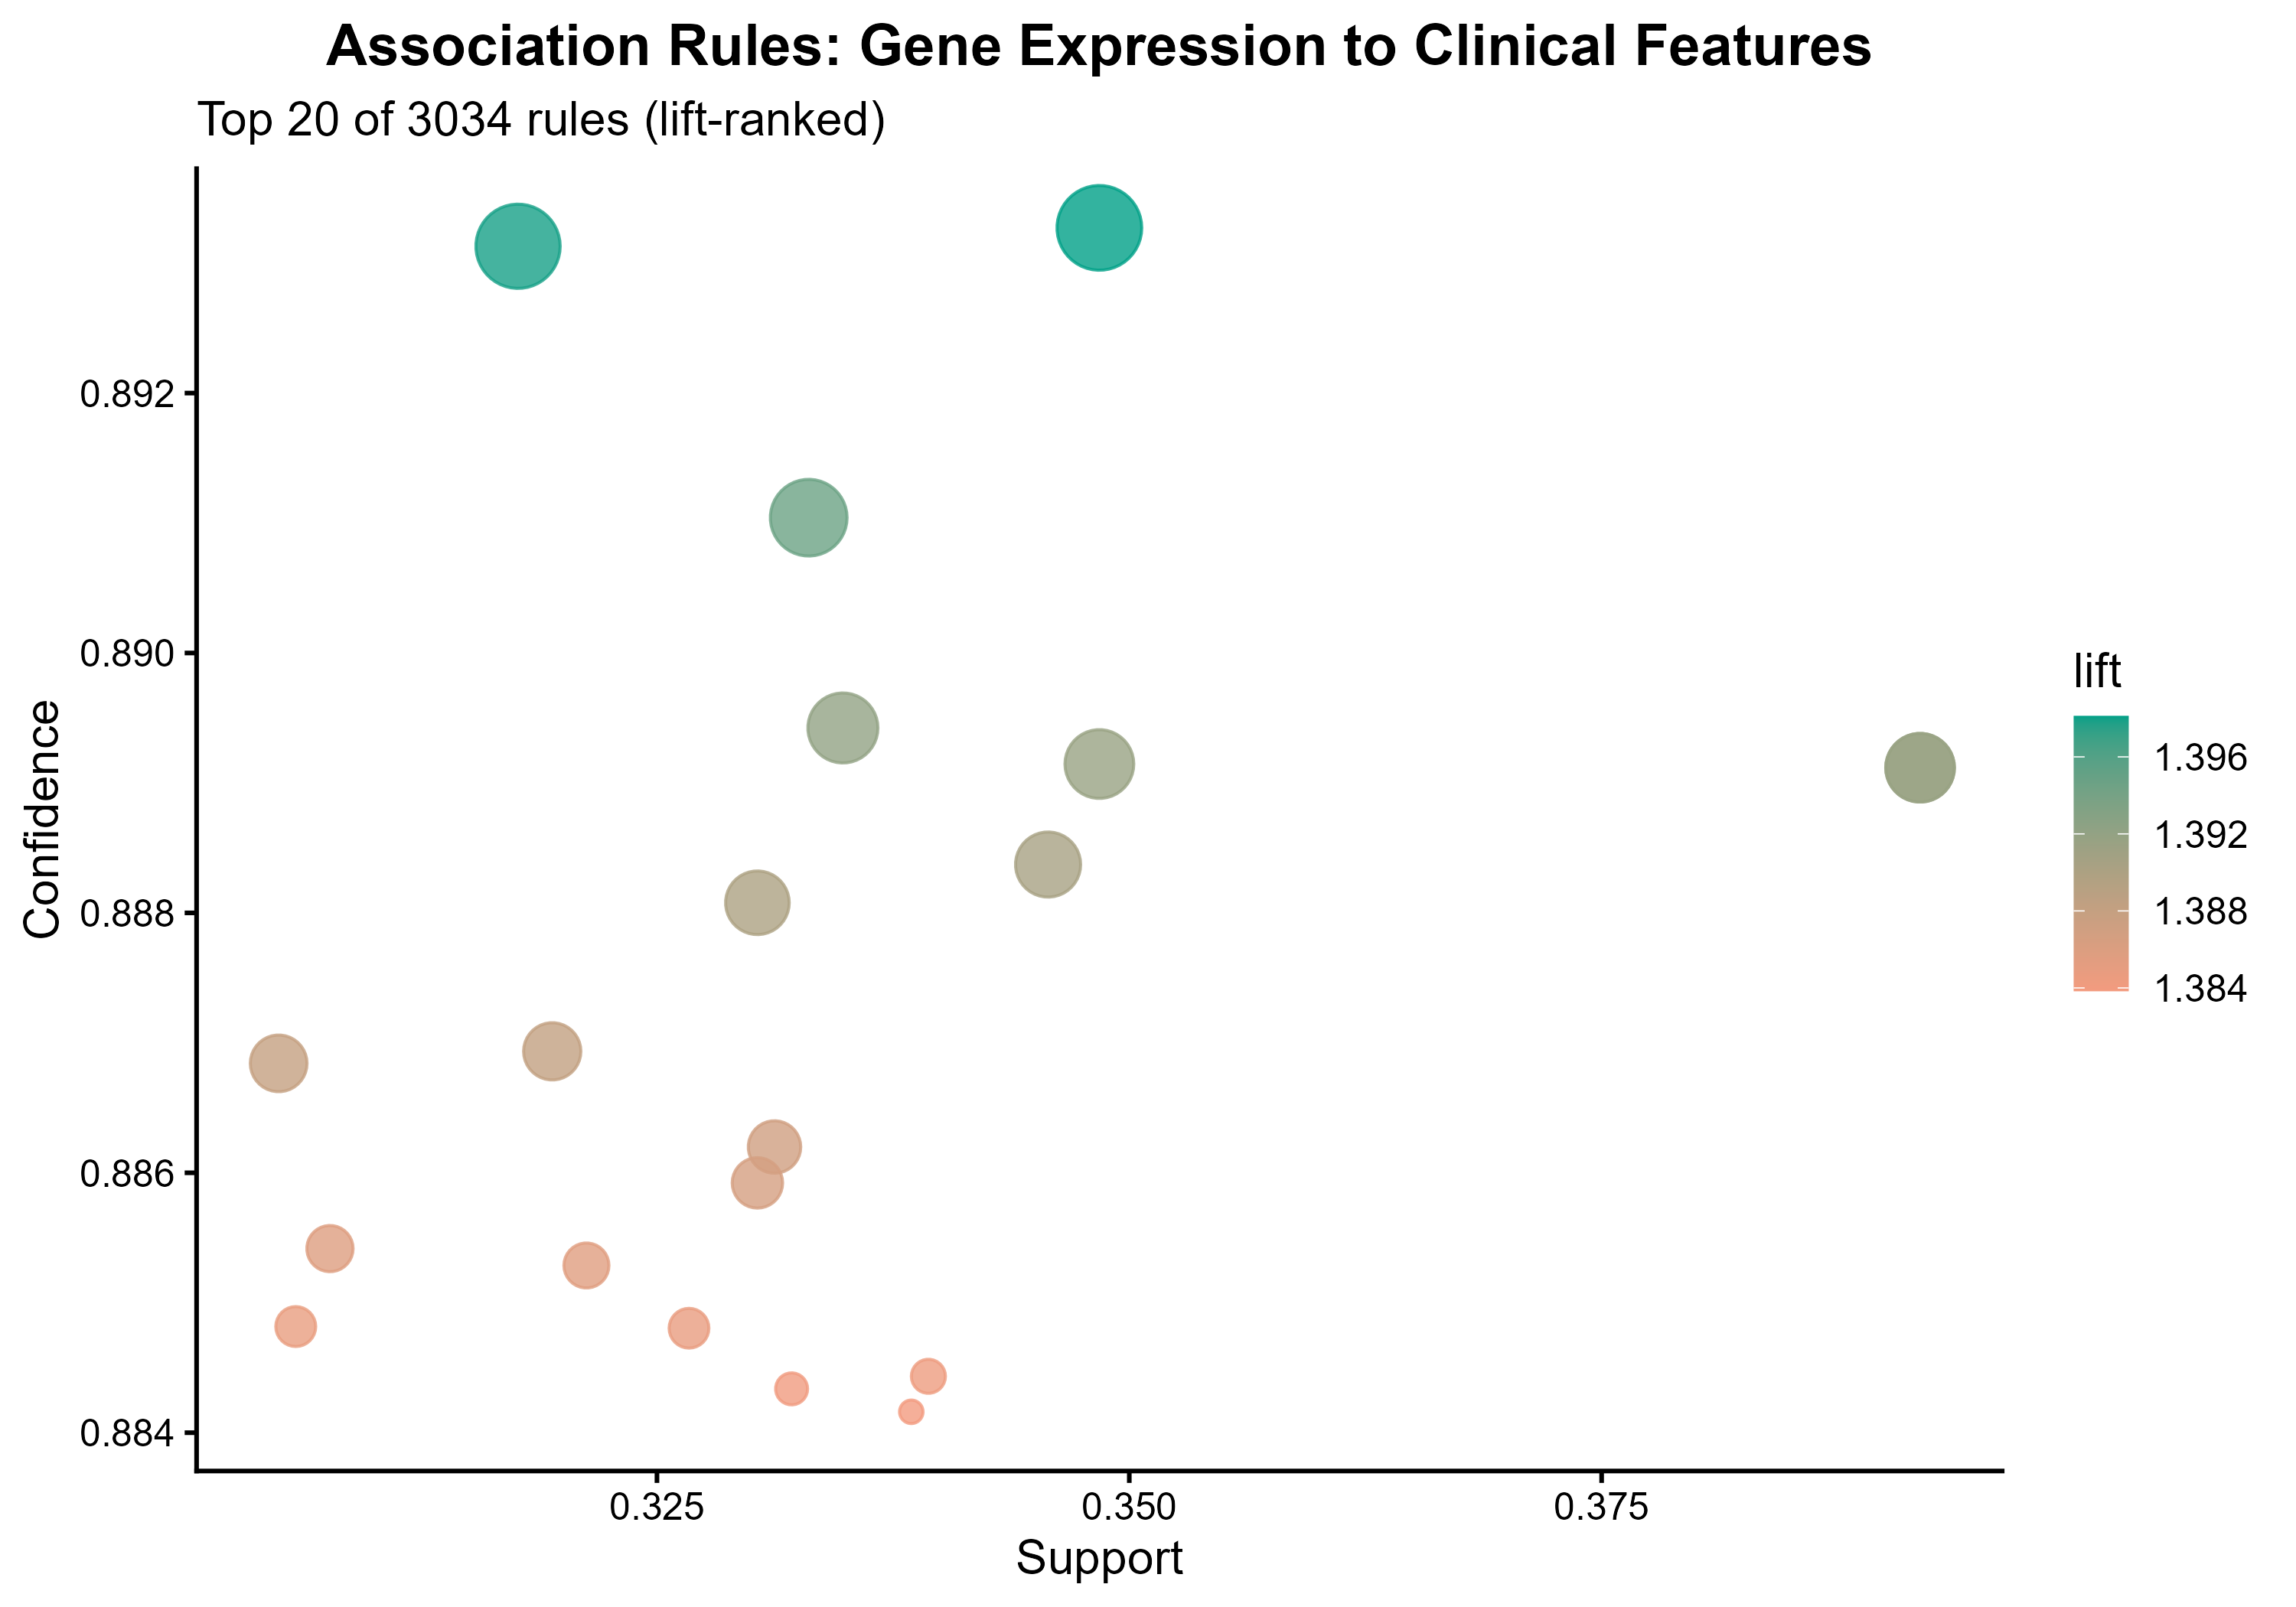
\includegraphics[width=0.8\textwidth]{fig15_association_rules.png}
\caption{关联规则散点图。横轴Support，纵轴Confidence，点大小和颜色编码Lift值。绘图参数：color gradient low=npg10[5]$\to$high=npg10[3]。Apriori算法，阈值support$\geq$0.3，confidence$\geq$0.7。}
\label{fig:rules}
\end{figure}

\begin{figure}[H]
\centering
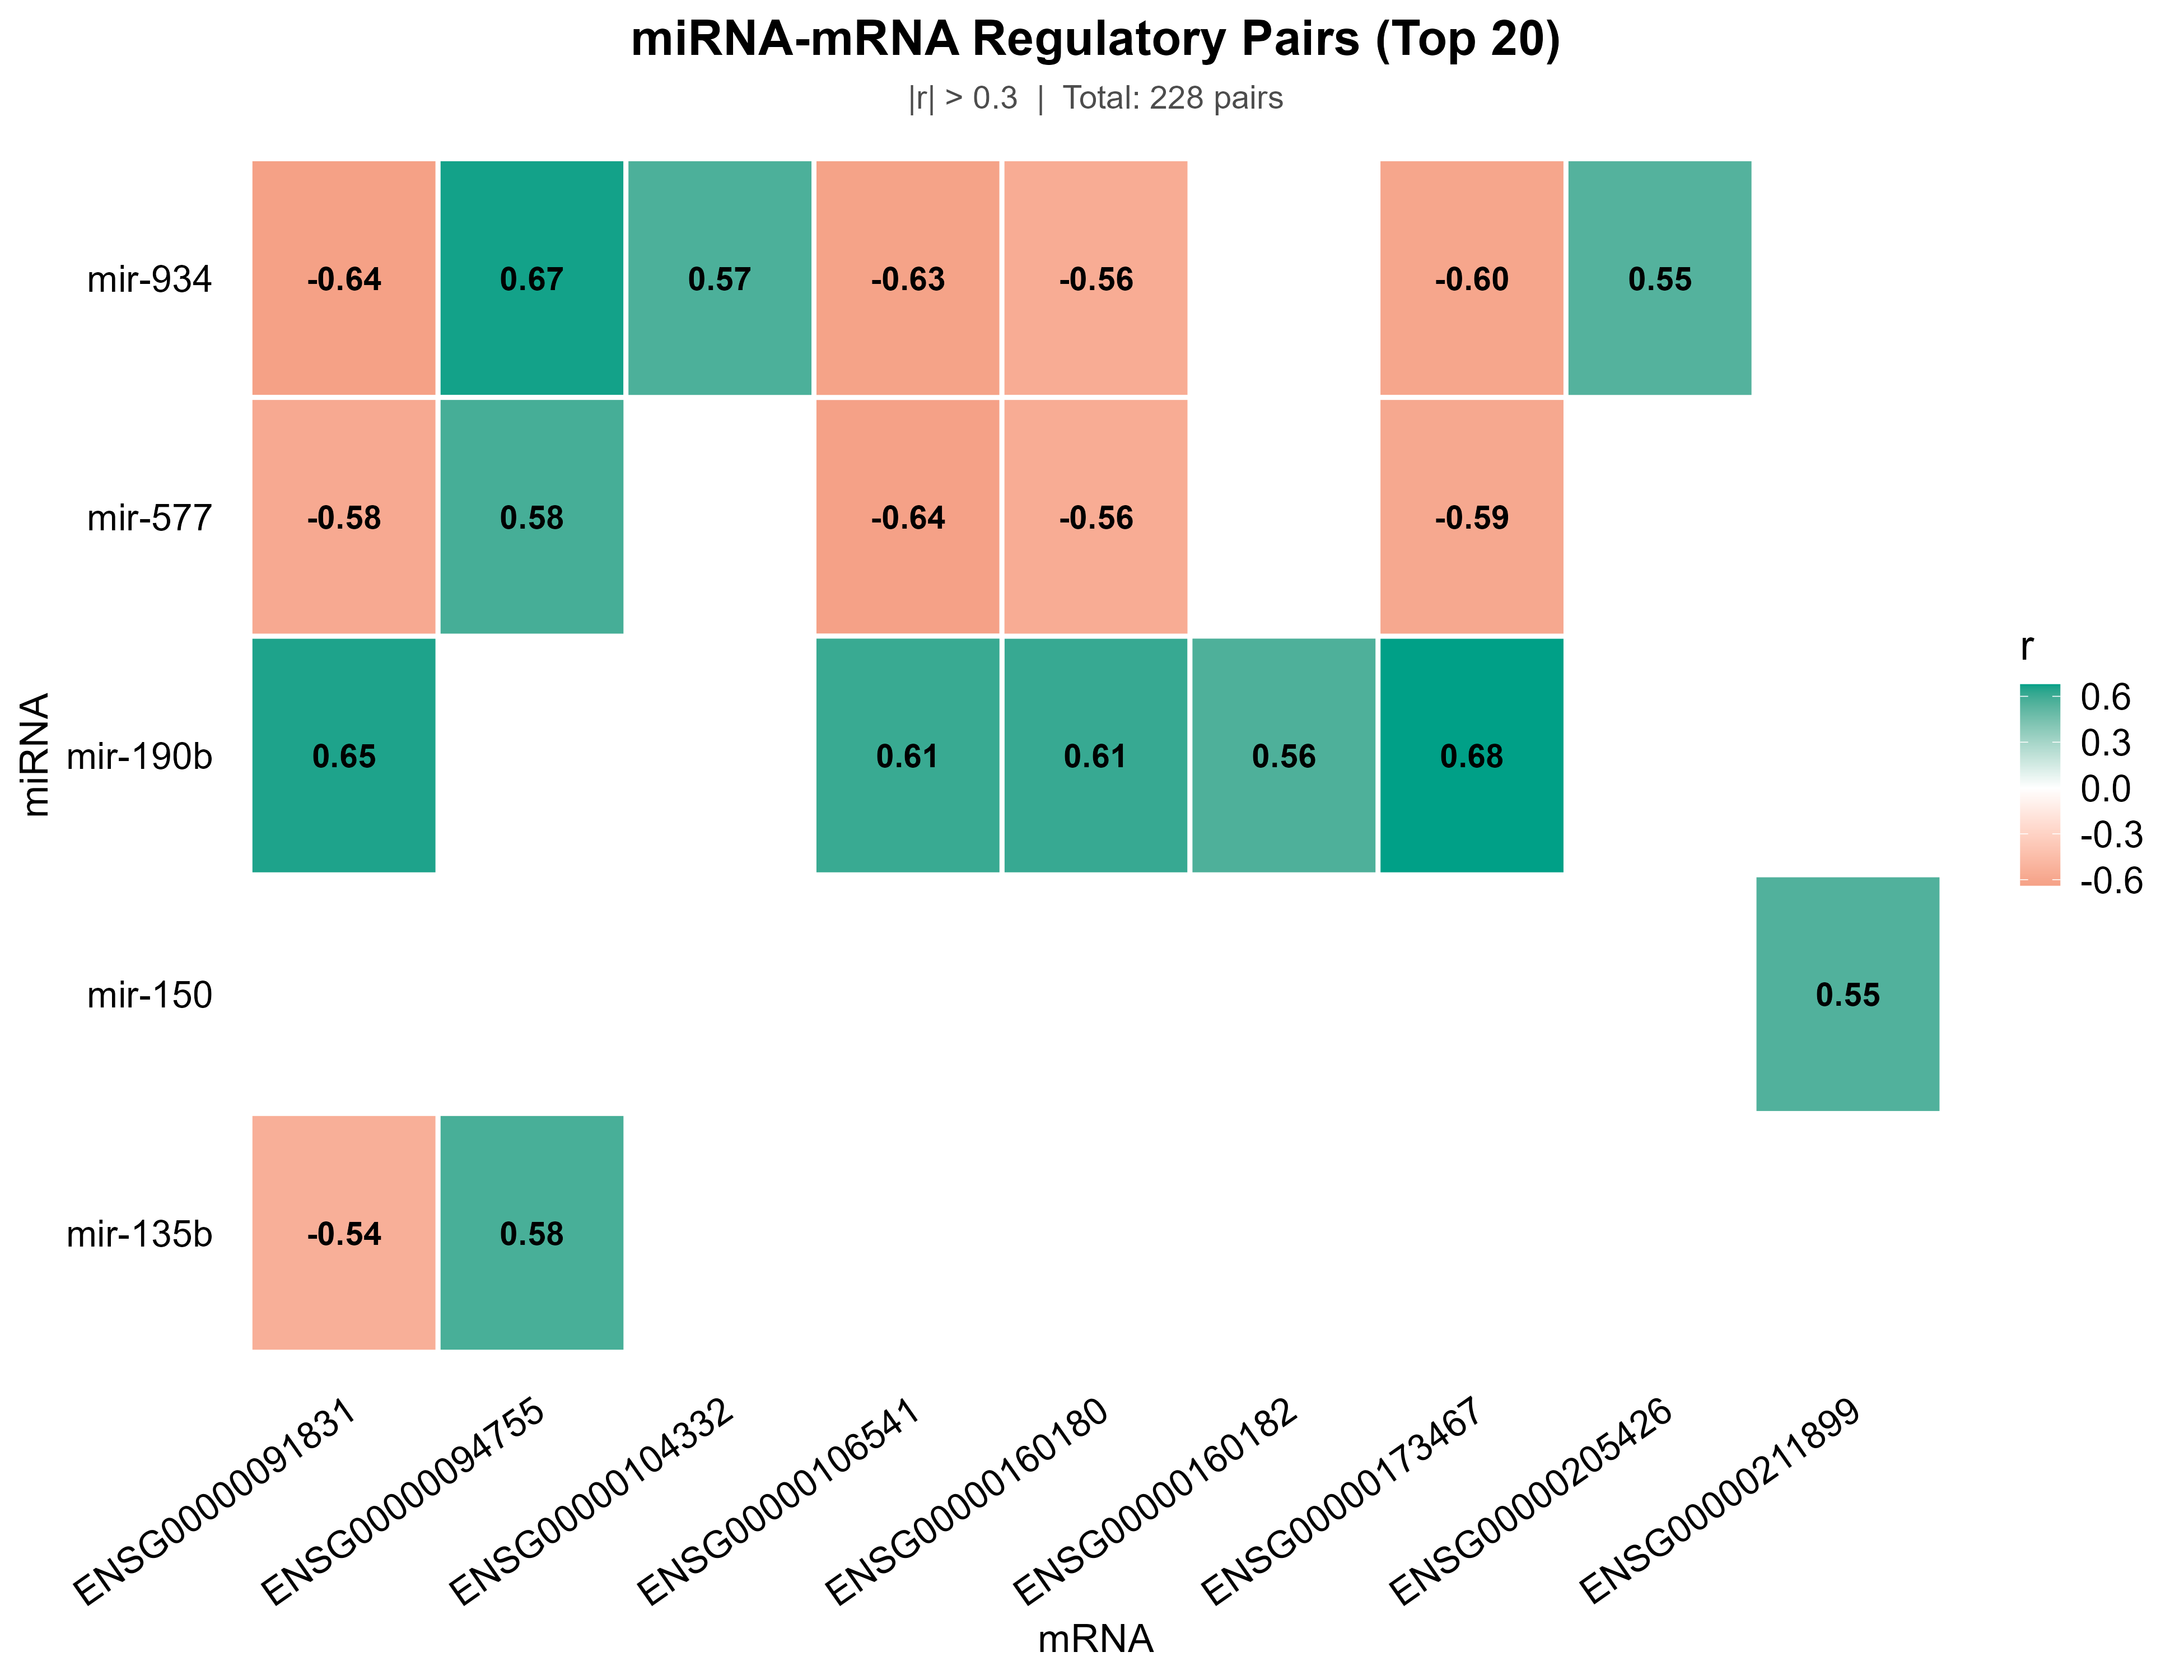
\includegraphics[width=0.85\textwidth]{fig10_mirna_mrna_corr.png}
\caption{miRNA-mRNA调控相关性热图（Top 20, $|r|>0.4$）。行=miRNA, 列=mRNA, 格内标注Pearson $r$值。色阶：scale\_fill\_gradient2(low=npg10[5], mid=white, high=npg10[3])。}
\label{fig:mirna}
\end{figure}

% ==================== 4 讨论 ====================
\section{讨论}

本研究通过系统的多组学数据挖掘，构建了覆盖11种分析方法的BRCA分子特征整合分析管线。

\textbf{差异表达与功能富集}：上调基因集中于细胞周期和DNA复制通路，下调基因集中于ECM组织和细胞黏附通路——这一功能分工与肿瘤的增殖活跃和微环境脱离特征高度吻合。Reactome Cell Cycle通路的富集显著性（$p=1.5\times10^{-21}$）远超其他通路，反映出细胞周期失调在BRCA转录组全局变化中的核心地位。上调条目中GO:BP贡献了最多条目数（303条）、Reactome贡献了最强的显著性（前五位全部来自Reactome）——这两个数据库的互补性说明综合使用多数据库富集并非冗余。TN与Luminal A之间存在4,888个差异表达基因，这一数字与Tumor vs Normal的6,768处于同一数量级，暗示亚型间转录组差异的幅度不亚于肿瘤正常差异。

\textbf{分类与聚类的一致性}：LASSO的高准确率（89.4\%）和低特征数（35个基因）共同验证了亚型间转录组差异的稀疏性。PCA、t-SNE和K-means三种独立方法一致指向ER状态为最显著的分组驱动因素，与分类分析中分子亚型的可预测性互为印证。PCA中PC1仅解释了15.3\%的方差，说明ER状态虽然是主导因素，但BRCA转录组的全局结构相当分散——绝大多数变异维度不与已知分类标签对齐。

\textbf{生存预后}：Cox模型在控制分期后分子亚型无独立预后贡献（所有$p>0.5$），与部分文献的结论存在分歧。可能原因：本队列随访时间较短（中位2.7年）、死亡事件有限（87例），以及不同亚型患者接受了针对性治疗部分抹平了固有预后差异。

\textbf{突变特征}：PIK3CA和TP53的高频突变及两者互斥趋势与已知BRCA驱动突变谱一致。TMB在Triple Negative中显著高于Luminal A（1.47 vs 0.79/Mb），这一差异可能部分解释TNBC对免疫检查点抑制剂的较高应答率——更高的TMB$\to$更多新抗原$\to$增强的抗肿瘤免疫。在BRCA这样的中等TMB癌种中，TMB的绝对值远低于黑色素瘤和肺癌，其作为免疫治疗预测标志物的价值需要结合具体阈值评估。

\textbf{局限性}：（1）DNA甲基化数据（450K, 11.7 GB）未纳入分析；（2）生存事件率较低（7.9\%）限制了预后模型统计功效；（3）miRNA-mRNA调控基于相关而非因果验证；（4）XGBoost未经系统超参数调优。

% ==================== 5 结论 ====================
\section{结论}

本研究以TCGA-BRCA多组学数据为基础，整合mRNA、miRNA和体细胞突变三个组学层次，构建了覆盖差异表达分析、功能富集、分子亚型分类、聚类分析、WGCNA共表达网络、生存分析、突变分析、关联规则挖掘和miRNA调控网络分析的完整数据挖掘流程。主要结论如下：

（1）鉴定6,768个Tumor vs Normal及4,888个TN vs Luminal A差异表达基因。功能富集揭示上调基因集中于细胞周期通路（$p=1.5\times10^{-21}$），下调基因集中于ECM组织通路。

（2）LASSO以89.4\%准确率仅用35个基因实现三分类分子亚型预测，验证了亚型间转录组差异的稀疏性。

（3）PCA和K-means一致表明ER状态是BRCA转录组的最强驱动因素。

（4）WGCNA识别9个共表达模块，Blue模块枢纽基因MM达0.959。

（5）Cox模型C-index=0.771，Stage IV HR=8.74。

（6）PIK3CA（37.3\%）和TP53（35.2\%）为最高频突变基因。TN的TMB为Luminal A的1.86倍。

未来方向：纳入DNA甲基化数据实现四组学整合、独立队列外部验证、Blue模块枢纽基因功能实验、以及深度学习方法在多组学数据融合中的应用探索。

% ==================== 参考文献 ====================
\printbibliography

% ==================== 附录 ====================
\newpage
\appendix
\section{核心R代码}

以下附录收录本研究中全部关键分析步骤的R代码。

\subsection{数据预处理与差异表达分析}
\begin{lstlisting}[caption={01\_data\_preprocessing.R + 04\_diff\_expression.R}, basicstyle=\ttfamily\scriptsize]
# --- mRNA Preprocessing ---
brca <- readRDS("data/processed/brca_tumor_processed.rds")
counts_tumor  <- brca$counts
counts_normal <- readRDS("data/processed/brca_normal_counts.rds")
tpm_tumor <- brca$tpm
clinical  <- brca$clinical

# --- DESeq2: Tumor vs Normal ---
dds <- DESeqDataSetFromMatrix(
  countData = cbind(counts_tumor, counts_normal),
  colData   = data.frame(condition = factor(
    c(rep("Tumor", ncol(counts_tumor)),
      rep("Normal", ncol(counts_normal))))),
  design = ~ condition)
dds <- DESeq(dds)
res <- results(dds, contrast = c("condition", "Tumor", "Normal"), alpha = 0.05)
deg_table <- data.frame(gene = rownames(res), log2FC = res$log2FoldChange,
  pvalue = res$pvalue, padj = res$padj)

# --- Subtype DEG: TN vs Luminal A ---
dds_tnla <- DESeqDataSetFromMatrix(
  round(counts[, subtype_vec %in% c("Triple Negative","Luminal A")]),
  data.frame(subtype = factor(subtype_vec)),
  ~ subtype)
dds_tnla <- DESeq(dds_tnla)
res_tnla <- results(dds_tnla,
  contrast = c("subtype","Triple Negative","Luminal A"))
\end{lstlisting}

\subsection{功能富集分析}
\begin{lstlisting}[caption={g:Profiler enrichment}, basicstyle=\ttfamily\scriptsize]
library(gprofiler2)
enrich_up <- gost(query = up_genes, organism = "hsapiens",
  sources = c("GO:MF","GO:BP","GO:CC","KEGG","REAC","WP"),
  correction_method = "fdr", user_threshold = 0.05,
  exclude_iea = TRUE, evcodes = TRUE)
# Source distribution (up): GO:BP 303, REAC 191, GO:CC 75, GO:MF 37, WP 21, KEGG 16
\end{lstlisting}

\subsection{分子亚型分类}
\begin{lstlisting}[caption={05\_classification.R}, basicstyle=\ttfamily\scriptsize]
library(glmnet); library(randomForest)
# Feature selection: top 500 variable genes from log2(TPM+1)
# Train/test: 7:3 stratified split, 3 classes (LA/HER2/TN)
cv_fit <- cv.glmnet(X_train, y_train, family = "multinomial",
  alpha = 1, nfolds = 5)
lasso_pred <- predict(cv_fit, X_test, s = "lambda.min", type = "class")
# LASSO: Accuracy 0.894, Kappa 0.528, 35 genes selected

rf <- randomForest(X_train, y_train, ntree = 500)
rf_pred <- predict(rf, X_test)
# RF: Accuracy 0.867, Kappa 0.365, F1 Macro 0.706
\end{lstlisting}

\subsection{聚类分析}
\begin{lstlisting}[caption={06\_clustering.R}, basicstyle=\ttfamily\scriptsize]
# PCA: prcomp, top 2000 variable genes, center+scale
pca <- prcomp(t(log2(tpm[top2000, ] + 1)), center = TRUE, scale. = TRUE)
# PC1 15.3%, PC2 8.5%

# t-SNE: Rtsne(perplexity=30, max_iter=1000)

# K-means: silhouette scores for K=2-10 (25 starts each)
# Best K=2, silhouette=0.18

# Consensus clustering: ConsensusClusterPlus, 80% resampling, 1000 iterations
\end{lstlisting}

\subsection{WGCNA共表达网络}
\begin{lstlisting}[caption={08\_wgcna.R}, basicstyle=\ttfamily\scriptsize]
library(WGCNA); enableWGCNAThreads(4)
log_tpm <- log2(tpm_mat + 1)
gene_var <- apply(log_tpm, 1, var)
top5000 <- names(sort(gene_var, decreasing = TRUE))[1:5000]
datExpr <- t(log_tpm[top5000, ])

sft <- pickSoftThreshold(datExpr, powerVector = 1:20,
  networkType = "signed")
# Power=8, scale-free R^2=0.887

net <- blockwiseModules(datExpr, power = 8, TOMType = "signed",
  minModuleSize = 30, mergeCutHeight = 0.25, numericLabels = TRUE)
# 9 modules identified
module_colors <- labels2colors(net$colors)
hub_kME <- cor(datExpr, net$MEs)
\end{lstlisting}

\subsection{生存分析}
\begin{lstlisting}[caption={11\_survival\_analysis.R}, basicstyle=\ttfamily\scriptsize]
library(survival); library(rms)
# KM curves
fit <- survfit(Surv(os_years, vital_status) ~ stage_simple, data = clin)
# log-rank p < 0.0001

# Multivariate Cox
cox_model <- coxph(Surv(os_years, vital_status) ~
  age + lymph_nodes + stage + subtype, data = clin)
# C-index = 0.771, LR p = 8.62e-12
# Stage IV HR = 8.74 (95%CI 3.61-21.14, p<0.001)

# Nomogram (3-year survival)
dd <- datadist(clin); options(datadist = "dd")
cox_nomo <- cph(Surv(os_years, vital_status) ~ stage + age,
  data = clin, surv = TRUE, time.inc = 3)
nomogram(cox_nomo, fun = function(x) 1 - x,
  funlabel = "3-Year Survival Probability")
\end{lstlisting}

\subsection{突变分析与TMB}
\begin{lstlisting}[caption={12\_advanced\_algorithms.R + 20b\_tmb\_fix.R}, basicstyle=\ttfamily\scriptsize]
library(maftools)
maf <- read.maf("brca_mutations_temp.maf")
# 990 samples, 15,413 genes, 67,546 variants
# Top: PIK3CA 369 (37.3%), TP53 348 (35.2%), TTN 268 (27.1%)
oncoplot(maf, top = 12)

# TMB (WES ~38 Mb exome)
tmb <- maf@data %>%
  group_by(Tumor_Sample_Barcode) %>%
  summarise(TMB = n() / 38, .groups = "drop")
# TN median TMB 1.47/Mb vs Luminal A 0.79/Mb (1.86x)
\end{lstlisting}

\subsection{关联规则与miRNA调控网络}
\begin{lstlisting}[caption={07\_association\_analysis.R + 12\_advanced\_algorithms.R}, basicstyle=\ttfamily\scriptsize]
library(arules)
# Build transaction data: Top 50 DEGs (High/Low) + clinical features
trans <- as(items_list, "transactions")
rules <- apriori(trans,
  parameter = list(supp = 0.3, conf = 0.7, minlen = 2, maxlen = 4))

# miRNA-mRNA Pearson correlation
mirna_aligned <- readRDS("data/processed/brca_miRNA_aligned.rds")
mRNA_aligned  <- readRDS("data/processed/brca_mRNA_aligned.rds")
mirna_mrna_cor <- cor(t(mirna_aligned), t(mRNA_aligned))
# 2,065 pairs with |r| > 0.4
\end{lstlisting}

\subsection{数据下载}
\begin{lstlisting}[caption={02\_download\_mirna.R + 02\_download\_mutations.R}, basicstyle=\ttfamily\scriptsize]
library(TCGAbiolinks)
# miRNA
query <- GDCquery(project = "TCGA-BRCA",
  data.category = "Transcriptome Profiling",
  data.type = "miRNA Expression Quantification",
  workflow.type = "BCGSC miRNA Profiling")
GDCdownload(query, method = "api", files.per.chunk = 20)
mirna_data <- GDCprepare(query)

# Somatic mutations
query <- GDCquery(project = "TCGA-BRCA",
  data.category = "Simple Nucleotide Variation",
  data.type = "Masked Somatic Mutation",
  workflow.type = "Aliquot Ensemble Somatic Variant Merging and Masking")
GDCdownload(query, method = "api", files.per.chunk = 20)
maf_data <- GDCprepare(query)
\end{lstlisting}

\end{document}
